\chapter{优化问题与解}
\label{chap:optimization}

一个车间要安排两种产品的产量，工时和原料都有限，老板希望利润尽量高。一组观测要用几个系数拟合，我们希望拟合误差尽量小。两件事的内容毫不相干，问的却是同一句话：在允许的选择里，哪一个最好？

把这句话当真，马上会遇到一串问题。允许的选择可能一个也没有；选择可能越来越好，好到没有尽头；也可能越来越接近某个水平，却总差一点到不了。即使最好的选择存在，它也许不止一个。站在一个洼地的底部，四周都比脚下高，山那边却可能有更深的谷。最后，计算机交出来的只是一个“差不多”的点，我们还要说清它差多少。

可以把整章想成在地形图上找最低点：图上的位置是候选，地面高度是要比较的量，有些区域禁止进入。各节依次回答上面的问题。第~\ref{sec:opt-formulation}节把任务写成数学对象，规定什么叫解，什么叫没有解。第~\ref{sec:opt-existence}节问解在什么条件下一定存在。第~\ref{sec:opt-properties}节比较两个候选之间的线段，回答洼地底部是不是最低处、最低点是不是只有一个。

前三节讨论的都是解本身。第~\ref{sec:opt-optimality}节转到实际判断：手里有一个候选点，只看它附近的导数信息，能断定什么。第~\ref{sec:opt-approximate}节处理算法真正交出的东西，比较衡量近似解的几种指标，并说明它们之间在什么条件下可以换算。这些语言和记号在全卷通用，后面每一章都在这个框架里提出自己的算法。

\section{优化问题的表述}
\label{sec:opt-formulation}

我们先要把“选最好的”这句话写到可以判断对错的程度。为此要说清在哪些候选里选、按什么标准比较，以及“选出来”究竟指什么。我们先看两个具体任务，再抽出共同的写法。

\paragraph{资源分配}
一个车间生产两种产品，产量分别记为$x_1,x_2$，单位是批。每批产品一的利润是$3$，产品二的利润是$2$。每批产品各用$1$个工时，每天共有$4$个工时；每批产品一用$2$份原料，产品二用$1$份，每天共有$6$份原料。产量不能为负。

车间能调整的只有$x_1,x_2$这两个数，把它们合成向量$\bm{x}=(x_1,x_2)^\top\in\mathbb{R}^2$。要比较的是利润$3x_1+2x_2$。允许的产量组合满足
\begin{equation}
 x_1+x_2\leq4,\qquad 2x_1+x_2\leq6,\qquad x_1\geq0,\qquad x_2\geq0.
 \label{eq:opt-resource-constraints}
\end{equation}

这里要的是利润最大，而全卷统一讨论最小化。两者只差一个符号：最大化$3x_1+2x_2$与最小化$-(3x_1+2x_2)$选出的产量相同，最大利润等于最小值的相反数。于是取
\begin{equation}
 f(\bm{x})=-(3x_1+2x_2).
 \label{eq:opt-resource-objective}
\end{equation}

把约束~\eqref{eq:opt-resource-constraints}画在平面上，四条直线围出图~\ref{fig:opt-resource-region}中的浅蓝色四边形，产量只能在其中选。虚线是利润相等的产量组合，线旁的数字是利润值，线越往右上利润越高。利润为$10$的线恰好擦过四边形的一个角$(2,2)$，再往外推，线上就没有允许的点了。

\begin{BookInlineFigure}
  \centering
  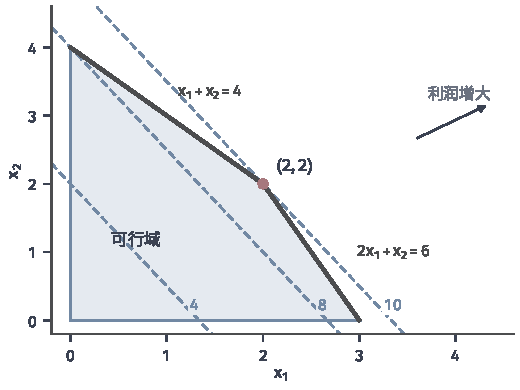
\includegraphics[width=88mm]{figures/05-optimization/01-linear-programming/matplotlib/opt-resource-region/figure.pdf}
  \caption{资源分配问题。浅蓝色四边形是全部允许的产量组合，顶点为$(0,0),(3,0),(2,2),(0,4)$；深灰粗线是工时约束与原料约束的边界。蓝色虚线是利润等于$4,8,10$的直线，红点$(2,2)$是利润为$10$的线与四边形唯一的公共点。}
  \label{fig:opt-resource-region}
\end{BookInlineFigure}

\paragraph{二次拟合}
第二个任务来自数据。设有$N$个观测和$n$个待定系数，矩阵$\bm{A}\in\mathbb{R}^{N\times n}$的第$i$行记录第$i$个观测的输入，向量$\bm{b}\in\mathbb{R}^N$记录观测值。系数$\bm{x}\in\mathbb{R}^n$给出的预测是$\bm{A}\bm{x}$，我们用平方误差比较不同的系数：
\begin{equation}
 f(\bm{x})=\frac12\lVert\bm{A}\bm{x}-\bm{b}\rVert_2^2+\frac{\gamma}{2}\lVert\bm{x}\rVert_2^2,\qquad\gamma\geq0.
 \label{eq:opt-ridge}
\end{equation}
第一项衡量预测与观测的差距，第二项称为正则项，系数$\gamma$决定对大系数收多少“费”。这个目标是$\bm{x}$的二次函数，所以称为二次拟合。

全章反复使用一个最小的实例：只有一个观测，$N=1$；两个系数，$n=2$；$\bm{A}=(1\ \ 1)$，$\bm{b}=2$。它的含义是“只测到两个量的和约等于$2$”。此时
\begin{equation}
 f(\bm{x})=\frac12(x_1+x_2-2)^2+\frac{\gamma}{2}(x_1^2+x_2^2).
 \label{eq:opt-ridge-instance}
\end{equation}
这个例子小到可以手算，却已经包含解不唯一、平坦方向和误差指标互相矛盾这些现象。

\paragraph{统一的写法}
两个任务都是在一个集合里选$\bm{x}$，使一个数尽量小。我们把这个结构固定下来，并同时规定全卷的记号。

\begin{definition}[优化问题]
\label{def:opt-problem}
给定集合$\bm{C}\subseteq\mathbb{R}^n$与函数$f:\bm{C}\to\mathbb{R}$，寻找使$f$尽量小的$\bm{x}\in\bm{C}$的任务称为\term{优化问题}（optimization problem），写作
\begin{equation}
 \min_{\bm{x}\in\bm{C}}f(\bm{x}).
 \label{eq:opt-general}
\end{equation}
$\bm{x}$称为\term{决策变量}（decision variable），$f$称为\term{目标函数}（objective function），$\bm{C}$称为\term{可行集}（feasible set），$\bm{C}$中的点称为\term{可行点}（feasible point）。
\end{definition}

可行集常常由一组条件给出。全卷把不等式都整理成“$\leq0$”的形式，写作
\begin{equation}
 \bm{C}=\bigl\{\bm{x}\in\mathbb{R}^n:\ g_i(\bm{x})\leq0,\ i=1,\ldots,m;\ h_j(\bm{x})=0,\ j=1,\ldots,p\bigr\}.
 \label{eq:opt-constraint-form}
\end{equation}
其中$g_i$是不等式约束，共$m$个；$h_j$是等式约束，共$p$个。资源分配里没有等式约束，四个不等式约束是
\[
 g_1(\bm{x})=x_1+x_2-4,\quad g_2(\bm{x})=2x_1+x_2-6,\quad g_3(\bm{x})=-x_1,\quad g_4(\bm{x})=-x_2.
\]
二次拟合里没有约束，$\bm{C}=\mathbb{R}^n$。

$\bm{C}$与$f$必须一起给定，问题才算确定。对二次拟合而言，改变$\gamma$是在改变候选之间的比较标准，全部候选都还在；加上硬性要求$x_1\geq1.2$则是把一部分候选直接淘汰。前者像调整评分表，后者像修改参赛资格。两种改动都可能让答案变化，但机制不同，这一区别到本节末尾还会出现。

\paragraph{最优值与最优解}
“最低点”其实包含两个问题：最低的高度是多少，这个高度在哪里取得。前者是一个数，后者是一个位置。两者要分开定义，因为第一个问题有答案时，第二个问题可能没有。

\begin{definition}[最优值与最优解]
\label{def:opt-optimal-value}
问题~\eqref{eq:opt-general}的\term{最优值}（optimal value）是
\begin{equation}
 f^\star=\inf_{\bm{x}\in\bm{C}}f(\bm{x})\in[-\infty,+\infty],
 \label{eq:opt-optimal-value}
\end{equation}
并约定空集上的下确界为$+\infty$。若可行点$\bm{x}^\star$满足$f(\bm{x}^\star)=f^\star$，就称它为\term{最优解}（optimal solution）。全体最优解组成的集合记为$\argmin_{\bm{x}\in\bm{C}}f(\bm{x})$。这个集合非空时，称最优值被达到。
\end{definition}

符号$\min$在式~\eqref{eq:opt-general}中只表示提出任务。若有人写“最小值等于某个数”，他同时断言了这个数被某个可行点取得；若只知道下确界，应当写$\inf$。

现在解资源分配问题。要证明$(2,2)$最好，需要两件事：所有可行点的利润都不超过某个数，并且$(2,2)$达到了这个数。第一件事可以这样做：利润系数$(3,2)$恰好是两条资源约束系数$(1,1)$与$(2,1)$之和，所以对任意可行点，把两条约束相加，得到
\[
 3x_1+2x_2=(x_1+x_2)+(2x_1+x_2)\leq4+6=10.
\]

这说明$f(\bm{x})\geq-10$对所有可行点成立。等号成立当且仅当两条资源约束同时取等号，也就是
\[
 x_1+x_2=4,\qquad 2x_1+x_2=6.
\]
解得$\bm{x}=(2,2)$，它满足非负约束，因而可行。于是
\[
 f^\star=-10,\qquad \argmin_{\bm{x}\in\bm{C}}f(\bm{x})=\{(2,2)\}.
\]

这个论证的结构值得记住：一个对所有可行点成立的下界，加上一个达到该下界的可行点，从两侧把最优值夹住，两者缺一不可。只有下界，不知道它是否够紧；只有候选点，不知道还有没有更好的。第~\ref{chap:linear-programming}章会说明，“给约束配权重再相加”可以系统地做。

二次拟合实例~\eqref{eq:opt-ridge-instance}取$\gamma=0$时，$f(\bm{x})=\frac12(x_1+x_2-2)^2\geq0$。凡满足$x_1+x_2=2$的点都使$f=0$，所以$f^\star=0$，最优解是一整条直线。比如$(1,1)$和$(3,-1)$都最优。数据只约束了两个量的和，没有约束它们的差，参数不唯一并不是计算失败，而是问题本身没有提供区分它们的信息。

\paragraph{三种没有最优解的情形}
并不是每个问题都有解，失败有三种不同的方式，分别出在不同的环节。

\begin{itemize}
 \item \term{不可行}（infeasible）：$\bm{C}=\varnothing$，此时$f^\star=+\infty$。例如同时要求$x\leq0$与$x\geq1$。
 \item \term{无下界}（unbounded below）：$\bm{C}\neq\varnothing$且$f^\star=-\infty$。例如在$\mathbb{R}$上最小化$f(x)=x$，取$x=-k$可得$f=-k\to-\infty$。
 \item 下确界未达到：$f^\star$是有限实数，但$\argmin$为空。例如在$\mathbb{R}$上最小化$f(x)=e^x$。
\end{itemize}

第三种最容易被忽略。对$e^x$，处处有$e^x>0$，又有$e^{-k}\to0$，所以$f^\star=0$；但没有$x$使$e^x=0$。只报告“最优值是$0$”而不说明它未被达到，读者会以为存在一个最优的$x$。图~\ref{fig:opt-failure-modes}把三种情形放在一起。

\begin{BookInlineFigure}
  \centering
  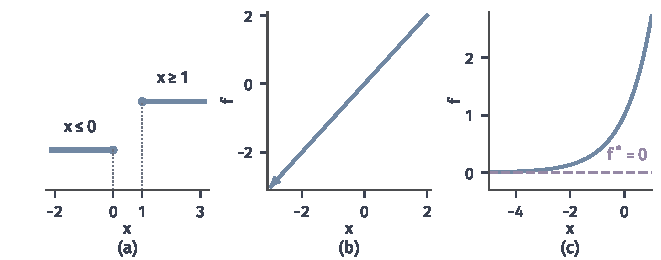
\includegraphics[width=112mm]{figures/05-optimization/01-linear-programming/matplotlib/opt-failure-modes/figure.pdf}
  \caption{优化问题没有最优解的三种方式。(a)约束$x\leq0$与$x\geq1$对应的两段蓝色射线没有公共点，可行集为空。(b)$f(x)=x$沿箭头方向无限下降，最优值为$-\infty$。(c)$f(x)=e^x$趋于紫色虚线$f^\star=0$却永远碰不到：最优值有限，但没有点取得它。}
  \label{fig:opt-failure-modes}
\end{BookInlineFigure}

\paragraph{局部最优与全局最优}
前面的最优解要和所有可行点比。实际计算时，我们往往只看得见当前点附近的情况，所以还需要一个只和附近比较的概念。“附近”用开球表示：
\[
 \bm{B}(\bm{x},r)=\{\bm{y}:\lVert\bm{y}-\bm{x}\rVert_2<r\}.
\]

\begin{definition}[局部最优解]
\label{def:opt-local}
设$\bm{x}^\star\in\bm{C}$。若存在$r>0$，使
\begin{equation}
 f(\bm{x}^\star)\leq f(\bm{x})\qquad\text{对所有}\ \bm{x}\in\bm{C}\cap\bm{B}(\bm{x}^\star,r)\ \text{成立},
 \label{eq:opt-local}
\end{equation}
就称$\bm{x}^\star$为\term{局部最优解}（local minimizer）。若对其中所有$\bm{x}\neq\bm{x}^\star$都有严格不等式，就称它为\term{严格局部最优解}（strict local minimizer）。定义~\ref{def:opt-optimal-value}中的最优解也称\term{全局最优解}（global minimizer）。
\end{definition}

比较的范围是$\bm{C}\cap\bm{B}(\bm{x}^\star,r)$，不是整个球。可行集边界上的点只需要和球内的可行点比较，球里伸出可行集的部分不参加比较。下面的例子同时展示洼地与边界。

\begin{example}[两个洼地与一个边界]
\label{ex:opt-local-global}
在可行集$\bm{C}=[-1.5,1.5]$上最小化
\[
 f(x)=\frac{x^4}{4}-\frac{x^3}{3}-x^2.
\]
先求导并分解因式：
\[
 f'(x)=x^3-x^2-2x=x(x-2)(x+1).
\]
所以$f'$在$x=-1,0,2$处为零。其中$x=2$在可行集之外。由$f'$的符号，$f$在$[-1.5,-1]$上递减，在$[-1,0]$上递增，在$[0,1.5]$上递减。

因此$x=-1$附近的可行点函数值都不低于$f(-1)$，它是局部最优解。$\bm{C}$上的最小值只可能出现在$x=-1$或右端点$x=1.5$，两处的函数值是
\[
 f(-1)=-\frac{5}{12}\approx-0.417,\qquad f(1.5)\approx-2.109.
\]
所以全局最优解是$x=1.5$。这一点在边界上，那里$f'(1.5)=-1.875\neq0$：函数还在向右下降，只是可行集不允许再往右走。
\end{example}

图~\ref{fig:opt-local-global}画出这个例子，地形的比喻在这里很贴切。黄点是一个洼地的底部，站在那里四周都更高，它却不是最低处。红点是真正的最低处，脚下的地面还是斜的，挡住我们的是边界，不是地形。可行集右侧还有更低的点$x=2$，但它不是候选，与问题无关。

\begin{BookInlineFigure}
  \centering
  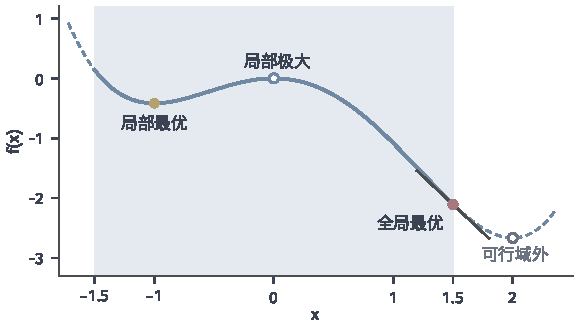
\includegraphics[width=98mm]{figures/05-optimization/01-linear-programming/matplotlib/opt-local-global/figure.pdf}
  \caption{$f(x)=x^4/4-x^3/3-x^2$在$\bm{C}=[-1.5,1.5]$（浅蓝色带）上的局部与全局最优。蓝色实线是$\bm{C}$上的图像，虚线是$\bm{C}$外的部分。黄点$x=-1$是局部最优解，红点$x=1.5$是全局最优解，该处的短切线不水平，斜率为$-1.875$。空心点分别是局部极大点$x=0$和可行集外的$x=2$。}
  \label{fig:opt-local-global}
\end{BookInlineFigure}

严格局部最优只说明一个小邻域内没有并列者，并不排除远处有同样低的点。函数$(x^2-1)^2$在$x=\pm1$处都取到全局最小值$0$，两点各自是严格局部最优解，全局最优解却有两个。

\paragraph{把约束并入目标}
到目前为止，可行集和目标是两个分开的对象。后面常要把几种代价相加，或者用同一个工具处理各种约束，分开写很不方便。一个自然的想法是：给不可行的点一个大到不可能被选中的值。任何有限的数都不够保险，所以我们允许函数取$+\infty$。

\begin{definition}[扩展实值函数与约束指标函数]
\label{def:opt-extended}
取值于$\mathbb{R}\cup\{+\infty\}$的函数称为\term{扩展实值函数}（extended real-valued function）。它的\term{有效定义域}（effective domain）是$\operatorname{dom}F=\{\bm{x}:F(\bm{x})<+\infty\}$；有效定义域非空时，称$F$为\term{适当函数}（proper function）。集合$\bm{C}\subseteq\mathbb{R}^n$的\term{约束指标函数}（constraint indicator function）是
\begin{equation}
 \iota_{\bm{C}}(\bm{x})=\begin{cases}0,&\bm{x}\in\bm{C},\\+\infty,&\bm{x}\notin\bm{C}.\end{cases}
 \label{eq:opt-constraint-indicator}
\end{equation}
扩展实值目标$F$的最优解集合规定为
\begin{equation}
 \argmin F=\{\bm{x}\in\operatorname{dom}F:F(\bm{x})=\inf F\}.
 \label{eq:opt-extended-argmin}
\end{equation}
\end{definition}

对可行集$\bm{C}$非空的问题，令$F=f+\iota_{\bm{C}}$，也就是在$\bm{C}$上$F=f$，在$\bm{C}$外$F=+\infty$。这里$f+\iota_{\bm{C}}$在$\bm{C}$外按$+\infty$理解，不要求$f$在那里有定义。逐项核对这种写法保留了什么。

首先，$\operatorname{dom}F=\bm{C}$，所以取有限值的候选恰好是可行点。其次，$F$与$f$在可行点上取值相同，其余点取$+\infty$，不影响下确界，于是
\[
 \inf_{\mathbb{R}^n}F=\inf_{\bm{x}\in\bm{C}}f(\bm{x}).
\]
最后，最优解只在$\operatorname{dom}F=\bm{C}$中找，所以$\argmin F$与原问题的最优解集合相同。若$\bm{C}=\varnothing$，则$F\equiv+\infty$不是适当函数，应报告不可行；定义中限定在$\operatorname{dom}F$内找解，正是为了避免说成“每一点都最优”。

\paragraph{约束指标函数不是普通指示函数}
名称相近的普通\term{指示函数}（indicator function）$\mathbb{1}_{\bm{C}}$在$\bm{C}$上取$1$，在$\bm{C}$外取$0$。两者的取值表放在一起，就能看出差别。

\begin{BookInlineTable}
  \centering
  \begin{tabular}{@{}lcc@{}}
    \toprule
     & $\bm{x}\in\bm{C}$ & $\bm{x}\notin\bm{C}$\\
    \midrule
    约束指标函数$\iota_{\bm{C}}$ & $0$ & $+\infty$\\
    普通指示函数$\mathbb{1}_{\bm{C}}$ & $1$ & $0$\\
    \bottomrule
  \end{tabular}
  \caption{约束指标函数与普通指示函数的取值。前者用于把违规点排除，后者只是记录一个点是否属于集合。}
  \label{tab:opt-indicators}
\end{BookInlineTable}

两者的方向也相反：$\iota_{\bm{C}}$在集合内为小值，$\mathbb{1}_{\bm{C}}$在集合内为大值。用一个例子看把它们加到目标上的后果。在约束$x\leq1$下最小化$(x-2)^2$，可行集记为$C=(-\infty,1]$。这个问题的最优解是$x=1$，最优值为$1$。

图~\ref{fig:opt-extended-value}比较三种加法。加$\iota_C$得到的问题就是原问题。加$\mathbb{1}_C$则让可行点反而贵了$1$，最小点跑到$x=2$，违反约束。

第三种是有限惩罚，它按违规程度收费。改为最小化$(x-2)^2+\max\{0,x-1\}$，在$x>1$的范围内令导数为零：
\[
 2(x-2)+1=0,\qquad x=1.5.
\]
此处函数值是$0.25+0.5=0.75$，低于约束问题的最优值$1$，所以惩罚问题的最小点违反了约束。

\begin{BookInlineFigure}
  \centering
  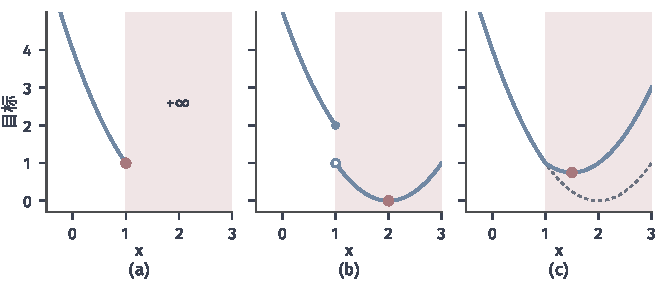
\includegraphics[width=112mm]{figures/05-optimization/01-linear-programming/matplotlib/opt-extended-value/figure.pdf}
  \caption{把约束$x\leq1$并入目标$(x-2)^2$的三种做法，浅红区域是不可行的点，红点是所得问题的最小点。(a)加约束指标函数，浅红区域取$+\infty$，最小点$x=1$与原问题相同。(b)加普通指示函数，可行点上升$1$，最小点变成不可行的$x=2$。(c)加有限惩罚$\max\{0,x-1\}$（灰色点线是原目标），最小点$x=1.5$仍不可行。}
  \label{fig:opt-extended-value}
\end{BookInlineFigure}

约束指标函数只是把同一个问题换了写法；有限惩罚改变了问题，只是不喜欢违规，并不禁止违规。惩罚要多大才能恢复约束，是第~\ref{chap:penalty-multiplier-methods}章的话题。今后需要时，我们把约束问题~\eqref{eq:opt-general}直接写成扩展实值目标的最小化，两种写法描述同一个问题。

\section{最优解的存在}
\label{sec:opt-existence}

$e^x$的例子说明，最优值有限并不保证有点取得它。于是要问：在什么条件下，可以不解问题就断定最优解存在？这个问题值得先回答。若解根本不存在，算法再怎么迭代也找不到它，“收敛”二字也就无从谈起。

\paragraph{从越来越好的候选出发}
设$\bm{C}$非空。按下确界的定义，总能取到一列可行点，使目标值趋于$f^\star$。若$f^\star$有限，就对每个$k$取可行点$\bm{x}^{(k)}$，使$f(\bm{x}^{(k)})\leq f^\star+1/k$；若$f^\star=-\infty$，就取$f(\bm{x}^{(k)})\leq-k$。这样的序列称为\term{最小化序列}（minimizing sequence）。上标$(k)$只是序列编号，这里还没有任何算法。

最小化序列的目标值越来越接近最优值，但序列本身可能乱跑。要从它得到一个最优解，需要依次通过三关：

\begin{enumerate}
 \item 序列留得住：存在收敛的子列，候选不会四散或逃向无穷远；
 \item 极限合法：子列的极限仍然是可行点；
 \item 比较能传到极限：极限处的目标值不高于序列目标值的极限。
\end{enumerate}

前两关由可行集负责，第三关由目标函数负责。图~\ref{fig:opt-existence-failures}中的三个例子各拆掉一关，绿点是最小化序列。

\begin{BookInlineFigure}
  \centering
  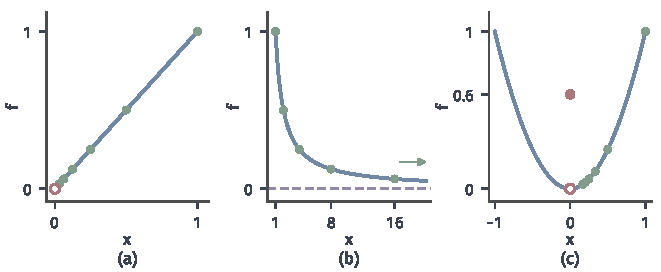
\includegraphics[width=112mm]{figures/05-optimization/01-linear-programming/matplotlib/opt-existence-failures/figure.pdf}
  \caption{存在性论证的三关分别失败。绿点是最小化序列。(a)$f(x)=x$，$C=(0,1]$：序列$2^{-k}$趋于不可行的端点$0$（红色空心点）。(b)$f(x)=1/x$，$C=[1,\infty)$：序列$2^k$逃向无穷远，目标值趋于紫色虚线$0$。(c)$f(x)=x^2$（$x\neq0$），$f(0)=0.6$，$C=[-1,1]$：序列$1/k$趋于$0$，目标值趋于$0$，而$f(0)$跳高到红点$0.6$，值$0$无人取得。}
  \label{fig:opt-existence-failures}
\end{BookInlineFigure}

(a)中$C=(0,1]$有界但不闭，序列有极限$0$，极限却被排除在外，第二关失败。(b)中$C=[1,\infty)$闭但无界，序列$2^k$没有收敛子列，第一关失败。(c)中$C=[-1,1]$很好，序列也收敛到可行点$0$，但函数在$0$处向上跳，极限处的值$0.6$高于序列目标值的极限$0$，第三关失败。

\paragraph{第一关与第二关：紧性}
在$\mathbb{R}^n$中，有界闭集的每个序列都有收敛子列，而且子列的极限仍在集合内。这样的集合称为\term{紧集}（compact set）。紧性恰好一次通过前两关：有界让序列留得住，闭让极限合法。有界闭集的这一性质及一般度量空间中的紧致性，可参考\BookChapterRef{chap:metric-spaces}{卷四第2章“度量空间”}。

\paragraph{第三关：只需要单向的比较}
第三关若用连续性通过，得到的是熟悉的结论：有界闭集上的连续函数取得最小值。仔细看却会发现，连续性要求多了。我们只需要极限处的值“不比序列高”，不需要它“等于序列的极限”。函数在极限点向下跳，只会让极限点更好；不能允许的是向上跳。

\begin{definition}[下半连续]
\label{def:opt-lsc}
设$\bm{C}\subseteq\mathbb{R}^n$，$f:\bm{C}\to\mathbb{R}\cup\{+\infty\}$。若对$\bm{C}$中每个收敛到$\bm{x}\in\bm{C}$的序列$\bm{x}^{(k)}$，都有
\begin{equation}
 f(\bm{x})\leq\liminf_{k\to\infty}f(\bm{x}^{(k)}),
 \label{eq:opt-lsc}
\end{equation}
就称$f$在$\bm{C}$上\term{下半连续}（lower semicontinuous）。
\end{definition}

连续函数满足这个条件且取等号。下半连续还可以用“高度不超过某个水平的部分”来刻画。对实数$a$，称
\begin{equation}
 \bm{S}_a=\{\bm{x}\in\bm{C}:f(\bm{x})\leq a\}
 \label{eq:opt-sublevel}
\end{equation}
为$f$的\term{下水平集}（sublevel set），也就是地形图上高度不超过$a$的区域。

图~\ref{fig:opt-lsc-sublevel}比较两个只在$x=0$一点取值不同的函数。左边$f(0)=0.4$，取跳跃下方的值，下半连续，高度不超过$0.6$的点组成闭区间$[0,0.4]$。右边$f(0)=1$，取跳跃上方的值，不下半连续，同一个下水平集是$(0,0.4]$，缺了左端点。右边的函数沿$x\downarrow0$可以无限接近$0.4$，却被$x=0$处的跳高挡住，最小值取不到。

\begin{BookInlineFigure}
  \centering
  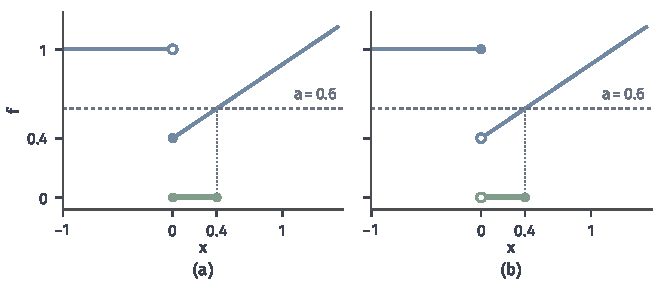
\includegraphics[width=112mm]{figures/05-optimization/01-linear-programming/matplotlib/opt-lsc-sublevel/figure.pdf}
  \caption{下半连续与下水平集的缺口。两个函数在$x<0$时都等于$1$，在$x>0$时都等于$0.4+0.5x$，实心蓝点是$x=0$处的函数值。灰色点线是水平$a=0.6$，绿色线段是下水平集$\bm{S}_{0.6}$。(a)$f(0)=0.4$，下半连续，下水平集是闭区间$[0,0.4]$。(b)$f(0)=1$，向上跳，下水平集$(0,0.4]$缺少左端点。}
  \label{fig:opt-lsc-sublevel}
\end{BookInlineFigure}

图中的观察就是下面的引理：下半连续性的作用，是让下水平集不缺边界。

\begin{lemma}[下半连续与闭下水平集]
\label{lem:opt-lsc-sublevel}
设$\bm{C}\subseteq\mathbb{R}^n$是闭集，$f:\bm{C}\to\mathbb{R}\cup\{+\infty\}$。$f$在$\bm{C}$上下半连续，当且仅当对每个$a\in\mathbb{R}$，下水平集$\bm{S}_a$是闭集。
\end{lemma}

\begin{proof}
先设$f$下半连续。取$\bm{S}_a$中的序列$\bm{x}^{(k)}$，设它收敛到$\bm{x}$。$\bm{C}$是闭集，所以$\bm{x}\in\bm{C}$。由下半连续性，
\[
 f(\bm{x})\leq\liminf_{k\to\infty}f(\bm{x}^{(k)})\leq a.
\]
所以$\bm{x}\in\bm{S}_a$，$\bm{S}_a$是闭集。

反过来，设每个$\bm{S}_a$都是闭集，但$f$在某点$\bm{x}\in\bm{C}$不满足式~\eqref{eq:opt-lsc}，即存在$\bm{C}$中收敛到$\bm{x}$的序列，使$\liminf_kf(\bm{x}^{(k)})<f(\bm{x})$。取实数$a$严格介于这两个量之间。下极限小于$a$，所以有子列$\bm{x}^{(k_j)}$始终满足$f(\bm{x}^{(k_j)})\leq a$，也就是子列落在$\bm{S}_a$中。

$\bm{S}_a$是闭集，子列的极限$\bm{x}$也在其中，于是$f(\bm{x})\leq a$。这与$a<f(\bm{x})$矛盾。
\end{proof}

\paragraph{紧可行集上的存在定理}
三关齐备，就得到第一个存在定理。

\begin{theorem}[紧可行集上的最小值]
\label{thm:opt-compact-existence}
设$\bm{C}\subseteq\mathbb{R}^n$非空且紧，$f:\bm{C}\to\mathbb{R}\cup\{+\infty\}$在$\bm{C}$上下半连续，且至少有一点取有限值。则最优值$f^\star$是有限实数，且最优解存在。
\end{theorem}

\begin{proof}
由假设，$f^\star<+\infty$。取一个最小化序列$\bm{x}^{(k)}\in\bm{C}$。$\bm{C}$是紧集，所以有子列$\bm{x}^{(k_j)}$收敛到某个$\bm{x}^\star\in\bm{C}$。由下半连续性，
\[
 f(\bm{x}^\star)\leq\liminf_{j\to\infty}f(\bm{x}^{(k_j)})=f^\star.
\]

若$f^\star=-\infty$，上式给出$f(\bm{x}^\star)=-\infty$，与$f$不取$-\infty$矛盾，所以$f^\star$有限。又因$\bm{x}^\star$可行，有$f(\bm{x}^\star)\geq f^\star$。两个不等式合起来得到
\[
 f(\bm{x}^\star)=f^\star.
\]
所以$\bm{x}^\star$是最优解。
\end{proof}

资源分配的可行集由四个闭半平面相交而成，它有界且闭，目标是线性函数，因而连续。定理~\ref{thm:opt-compact-existence}立刻保证最优解存在。这个结论不需要知道解在$(2,2)$，它只告诉我们值得去找。

定理的条件都是充分条件。例如$f(x)=x^2$的可行集$\mathbb{R}$无界，最小点$x=0$依然存在。图~\ref{fig:opt-existence-failures}的三个例子说明的是：逐条去掉条件后，结论可能不成立。

\paragraph{无界可行集：只看不太差的点}
二次拟合的可行集是整个$\mathbb{R}^n$，它不紧，定理~\ref{thm:opt-compact-existence}不能直接用。但我们并不需要整个可行集紧，只需要把最小化序列关进某个紧集。取一个有限的水平$a$，使下水平集$\bm{S}_a$非空。凡是目标值高于$a$的点都比$\bm{S}_a$中的点差，不可能是最优解，可以直接丢掉。剩下要看的只有$\bm{S}_a$。

\begin{theorem}[紧下水平集保证存在]
\label{thm:opt-compact-sublevel}
设$f:\bm{C}\to\mathbb{R}\cup\{+\infty\}$在$\bm{C}$上下半连续。若存在实数$a$，使下水平集$\bm{S}_a$非空且紧，则$f^\star$是有限实数，且最优解存在。
\end{theorem}

\begin{proof}
$f$限制在紧集$\bm{S}_a$上仍下半连续，并在$\bm{S}_a$上取有限值。由定理~\ref{thm:opt-compact-existence}，存在$\bm{x}^\star\in\bm{S}_a$，使$f(\bm{x}^\star)=\min_{\bm{S}_a}f\leq a$。

对$\bm{C}\setminus\bm{S}_a$中的点，有$f(\bm{x})>a\geq f(\bm{x}^\star)$。所以$\bm{x}^\star$是$f$在整个$\bm{C}$上的最小点，$f^\star=f(\bm{x}^\star)$有限。
\end{proof}

这个定理只要求有一个下水平集紧，其余的下水平集可以无界。在$\mathbb{R}$上考虑
\[
 f(x)=\frac{x^2}{1+x^2}.
\]
令$a=1/2$，解不等式$f(x)\leq1/2$，得到$x^2\leq1$，所以$\bm{S}_{1/2}=[-1,1]$是紧集，最小点$x=0$由此得到保证。而取$a\geq1$时，下水平集是整个$\mathbb{R}$，无界。

怎样检验下水平集紧？闭性由引理~\ref{lem:opt-lsc-sublevel}给出，只要$\bm{C}$闭、$f$下半连续。有界性则需要目标在远处足够高，这就是强制性。

\begin{definition}[强制性]
\label{def:opt-coercive}
设$\bm{C}\subseteq\mathbb{R}^n$，$f:\bm{C}\to\mathbb{R}\cup\{+\infty\}$。若对$\bm{C}$中任意满足$\lVert\bm{x}^{(k)}\rVert_2\to\infty$的序列，都有$f(\bm{x}^{(k)})\to+\infty$，就称$f$在$\bm{C}$上是\term{强制的}（coercive）。
\end{definition}

强制性等价于每个下水平集都有界。若某个$\bm{S}_a$无界，从中取范数趋于无穷的序列，其目标值始终不超过$a$，不满足强制性。反过来，若各下水平集都有界，而$\lVert\bm{x}^{(k)}\rVert_2\to\infty$，则对任意$a$，序列最终离开$\bm{S}_a$，也就是最终$f(\bm{x}^{(k)})>a$，所以$f(\bm{x}^{(k)})\to+\infty$。

于是得到实际最常用的形式：若$\bm{C}$非空闭，$f$下半连续且强制，并在$\bm{C}$上至少有一点取有限值，则最优解存在。这只需取$a$为该点的函数值，再用定理~\ref{thm:opt-compact-sublevel}。各条件的分工是：强制性使下水平集有界，留住了序列；$\bm{C}$闭与下半连续使下水平集闭，留住了极限。

\paragraph{回到二次拟合}
对式~\eqref{eq:opt-ridge}逐项核对。$f$是多项式，处处有限且连续；$\bm{C}=\mathbb{R}^n$是闭集。当$\gamma>0$时，拟合项非负，所以
\[
 f(\bm{x})\geq\frac{\gamma}{2}\lVert\bm{x}\rVert_2^2.
\]
范数趋于无穷时目标趋于无穷，$f$强制，最优解存在。

$\gamma=0$时情况不同。对实例~\eqref{eq:opt-ridge-instance}，沿方向$(1,-1)$目标不变：取$\bm{x}^{(k)}=(1+k,1-k)$，范数趋于无穷而$f=0$，所以$f$不强制。图~\ref{fig:opt-coercive-sublevel}比较了两种情形，同一个水平$a=1$的下水平集，在$\gamma=0$时是无界的带，在$\gamma=0.5$时收缩成一个椭圆。

\begin{BookInlineFigure}
  \centering
  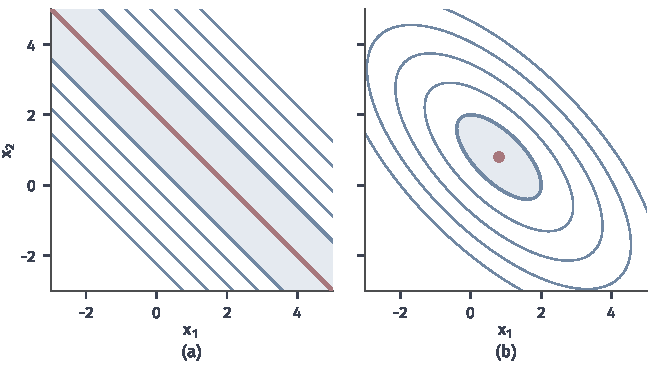
\includegraphics[width=112mm]{figures/05-optimization/01-linear-programming/matplotlib/opt-coercive-sublevel/figure.pdf}
  \caption{二次拟合实例$f(\bm{x})=\frac12(x_1+x_2-2)^2+\frac{\gamma}{2}\lVert\bm{x}\rVert_2^2$的下水平集。浅蓝区域及其粗边界是$\{f\leq1\}$，细线是其他等高线。(a)$\gamma=0$：下水平集是两条平行线之间的无界带，红线$x_1+x_2=2$是最优解集合。(b)$\gamma=0.5$：下水平集是椭圆，红点是唯一最优解$(0.8,0.8)$。}
  \label{fig:opt-coercive-sublevel}
\end{BookInlineFigure}

然而$\gamma=0$时最优解仍然存在，整条直线$x_1+x_2=2$都是。这再次说明强制性只是充分条件。对一般的$\bm{A}$，不带正则项的最小二乘总有解，依据是正规方程$\bm{A}^\top\bm{A}\bm{x}=\bm{A}^\top\bm{b}$总可解，可参考\BookChapterRef{chap:linear-solution-selection}{卷二第11章“线性方程与最小二乘的选解”}，这里用不到强制性。

\paragraph{有限维的边界}
整个论证依赖“有界闭集紧”，这是有限维空间的性质。平方可和的数列空间中，第$k$个坐标为$1$、其余为$0$的数列组成一列单位向量，它们两两距离都是$\sqrt2$，都在闭单位球里，却没有收敛子列。函数空间上的存在性要换一种收敛概念，第~\ref{chap:functional-optimization-variation}章会处理这件事；在$\mathbb{R}^n$中，本节的定理已经够用。

\section{解的性质}
\label{sec:opt-properties}

知道解存在之后，自然要问这个解是什么样的：洼地的底部是不是最低处？最低点是不是只有一个？目标值接近最优时，位置也接近吗？这些问题都在比较两个候选，最简单的比较路径是连接它们的线段。本节一路沿线段比较，逐步加强要求，依次回答这三个问题。

\paragraph{凸集：线段留在里面}
资源分配中，方案$\bm{u}=(3,0)$与$\bm{v}=(0,4)$都可行。各执行一半，得到混合方案$\frac12\bm{u}+\frac12\bm{v}=(1.5,2)$，它也可行，因为$1.5+2=3.5\leq4$，$3+2=5\leq6$，产量也非负。

这不是巧合。若$\bm{u},\bm{v}$都满足同一个线性不等式$\langle\bm{a},\bm{x}\rangle\leq c$，则对$\theta\in[0,1]$，
\[
 \langle\bm{a},\theta\bm{u}+(1-\theta)\bm{v}\rangle
 =\theta\langle\bm{a},\bm{u}\rangle+(1-\theta)\langle\bm{a},\bm{v}\rangle
 \leq\theta c+(1-\theta)c=c.
\]
可行方案任意混合仍然可行，这个性质值得单独命名。

\begin{definition}[凸集]
\label{def:opt-convex-set}
若对任意$\bm{u},\bm{v}\in\bm{C}$与$\theta\in[0,1]$，都有
\begin{equation}
 \theta\bm{u}+(1-\theta)\bm{v}\in\bm{C},
 \label{eq:opt-convex-set}
\end{equation}
就称$\bm{C}\subseteq\mathbb{R}^n$为\term{凸集}（convex set）。
\end{definition}

几何上，凸集里任意两点之间的线段都留在集合内。上面的计算说明半空间$\{\bm{x}:\langle\bm{a},\bm{x}\rangle\leq c\}$是凸集。若干凸集的交仍是凸集：两点同时在每个集合中，线段也同时在每个集合中。资源分配的可行集是四个半空间的交，所以是凸集。图~\ref{fig:opt-convex-sets}给出对照。

\begin{BookInlineFigure}
  \centering
  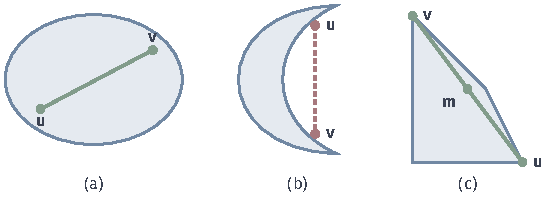
\includegraphics[width=93.691mm]{figures/05-optimization/01-linear-programming/tikz/opt-convex-sets/figure.pdf}
  \caption{凸集与非凸集。(a)椭圆盘中任意两点间的绿色线段留在集合内。(b)月牙形中两点都在集合里，红色虚线却穿过缺口，所以不是凸集。(c)资源分配的可行四边形，$\bm{u}=(3,0)$与$\bm{v}=(0,4)$的等权混合$\bm{m}=(1.5,2)$仍在集合内。}
  \label{fig:opt-convex-sets}
\end{BookInlineFigure}

\paragraph{凸函数：图像不鼓过弦}
可行集凸时，两个可行点之间的线段全是候选。接下来要求目标沿这条线段“不鼓起来”：线段上每一点的目标值，不超过两端目标值按相同权重的平均。

\begin{definition}[凸函数]
\label{def:opt-convex-function}
设$\bm{C}$为凸集。若$f:\bm{C}\to\mathbb{R}$对任意$\bm{u},\bm{v}\in\bm{C}$与$\theta\in[0,1]$满足
\begin{equation}
 f\bigl(\theta\bm{u}+(1-\theta)\bm{v}\bigr)\leq\theta f(\bm{u})+(1-\theta)f(\bm{v}),
 \label{eq:opt-convex-function}
\end{equation}
就称$f$为$\bm{C}$上的\term{凸函数}（convex function）。扩展实值函数称为凸函数，是指其有效定义域为凸集，且式~\eqref{eq:opt-convex-function}对有效定义域中的点成立。
\end{definition}

式~\eqref{eq:opt-convex-function}右端是连接两点$(\bm{u},f(\bm{u}))$与$(\bm{v},f(\bm{v}))$的弦上的点，左端是同一位置的函数值。所以凸函数的图像位于每条弦的下方，也就是碗的形状。图~\ref{fig:opt-chord}(a)是凸函数$x^2/2$；(b)中的函数有两个碗，连接两侧的弦从中间的鼓包下面穿过，不等式被破坏。对$F=f+\iota_{\bm{C}}$，这个定义恰好要求$\bm{C}$凸且$f$在$\bm{C}$上凸。

\begin{BookInlineFigure}
  \centering
  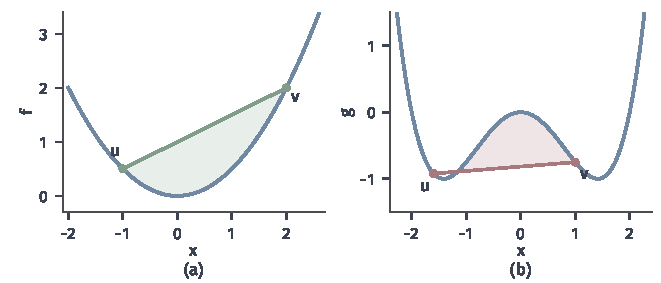
\includegraphics[width=112mm]{figures/05-optimization/01-linear-programming/matplotlib/opt-chord/figure.pdf}
  \caption{图像与弦。(a)凸函数$f(x)=x^2/2$，连接$x=-1$与$x=2$的绿色弦位于图像上方，浅绿区域是两者的间隔。(b)非凸函数$g(x)=x^4/4-x^2$，连接$x=-1.6$与$x=1$的红色弦有一段位于图像下方，浅红区域就是违反凸性的部分。}
  \label{fig:opt-chord}
\end{BookInlineFigure}

二次函数的情形可以算到底。设$\bm{H}\in\mathbb{R}^{n\times n}$对称，考虑
\[
 q(\bm{x})=\frac12\bm{x}^\top\bm{H}\bm{x}+\bm{a}^\top\bm{x}+a_0.
\]
记$\bm{w}=\theta\bm{u}+(1-\theta)\bm{v}$，我们计算弦与函数之间的间隔。线性项和常数项在加权平均中抵消，只需展开二次项：
\[
 \bm{w}^\top\bm{H}\bm{w}=\theta^2\bm{u}^\top\bm{H}\bm{u}+2\theta(1-\theta)\bm{u}^\top\bm{H}\bm{v}+(1-\theta)^2\bm{v}^\top\bm{H}\bm{v}.
\]

用$\theta-\theta^2=\theta(1-\theta)$，以及$(1-\theta)-(1-\theta)^2=\theta(1-\theta)$，得到
\begin{equation}
 \theta q(\bm{u})+(1-\theta)q(\bm{v})-q(\bm{w})=\frac12\theta(1-\theta)(\bm{u}-\bm{v})^\top\bm{H}(\bm{u}-\bm{v}).
 \label{eq:opt-quadratic-gap}
\end{equation}
所以$q$凸当且仅当$\bm{H}$半正定。

二次拟合目标~\eqref{eq:opt-ridge}展开后正是这种形式，其中$\bm{H}=\bm{A}^\top\bm{A}+\gamma\bm{I}$。对任意$\bm{w}$，
\[
 \bm{w}^\top\bm{H}\bm{w}=\lVert\bm{A}\bm{w}\rVert_2^2+\gamma\lVert\bm{w}\rVert_2^2\geq0,
\]
所以目标是凸函数。资源分配的目标是线性函数，式~\eqref{eq:opt-convex-function}取等号，也是凸函数。

\paragraph{局部最优就是全局最优}
现在回答第一个问题：山那边会不会有更深的谷。若目标和可行集都是凸的，答案是不会。

\begin{theorem}[凸问题的局部最优是全局最优]
\label{thm:opt-local-global}
设$\bm{C}$为凸集，$f:\bm{C}\to\mathbb{R}$为凸函数。则$f$在$\bm{C}$上的每个局部最优解都是全局最优解，并且最优解集合是凸集。
\end{theorem}

\begin{proof}
设$\bm{u}$是局部最优解，对应的邻域半径为$r$。假设存在$\bm{v}\in\bm{C}$使$f(\bm{v})<f(\bm{u})$。对$t\in(0,1)$，点$\bm{u}+t(\bm{v}-\bm{u})$在线段上，所以属于$\bm{C}$。由式~\eqref{eq:opt-convex-function}，
\[
 f\bigl(\bm{u}+t(\bm{v}-\bm{u})\bigr)\leq(1-t)f(\bm{u})+tf(\bm{v})<f(\bm{u}).
\]

取$t$足够小，使$t\lVert\bm{v}-\bm{u}\rVert_2<r$，这个更低的点就落在$\bm{C}\cap\bm{B}(\bm{u},r)$中，与局部最优矛盾。所以$\bm{u}$是全局最优解。

若$\bm{u},\bm{v}$都是最优解，线段上的点满足$f\leq\theta f^\star+(1-\theta)f^\star=f^\star$，也是最优解，所以最优解集合是凸集。
\end{proof}

证明的几何意义是：如果远处有更低的点，连向它的弦从当前点一出发就下降，凸函数的图像又在弦下方，紧贴当前点就有更低的点。图~\ref{fig:opt-local-implies-global}用非凸的例子~\ref{ex:opt-local-global}反过来看这件事：局部最优点$u$与更低的点$v$之间，弦在$u$的邻域里就低于$f(u)$，而图像却在弦上方，浅红区域正是对凸性的违反。

\begin{BookInlineFigure}
  \centering
  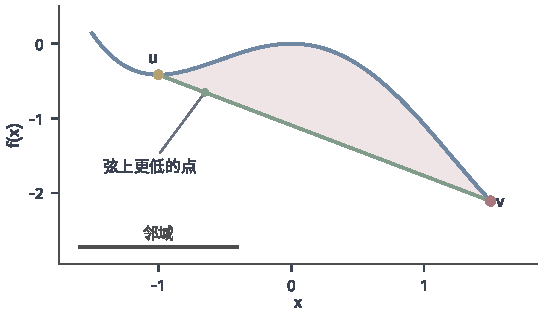
\includegraphics[width=92mm]{figures/05-optimization/01-linear-programming/matplotlib/opt-local-implies-global/figure.pdf}
  \caption{为什么凸问题没有假谷底。蓝线是$f(x)=x^4/4-x^3/3-x^2$，黄点$u=-1$是局部最优解，红点$v=1.5$更低。绿色弦上紧靠$u$的点已经低于$f(u)$，深灰线段是$u$的邻域。若$f$是凸函数，图像就必须在弦下方，$u$的邻域里就有更低的点；浅红区域表明这里的$f$不是凸函数，$u$才得以成为局部最优。}
  \label{fig:opt-local-implies-global}
\end{BookInlineFigure}

可行集和目标两个条件都要有。可行集不凸时，线段会跑出去：在$C=[-3,-1]\cup[1,3]$上最小化凸函数$(x-2)^2$，$x=-1$处的值是$9$，它的邻域里的可行点都在$[-3,-1]$中，函数值都不低于$9$，所以它是局部最优解；全局最优解却是$x=2$，值为$0$。目标不凸时，例子~\ref{ex:opt-local-global}已经给出反例。

\paragraph{严格凸与唯一性}
凸性排除了假谷底，但没有排除平坦的谷底：$\gamma=0$的拟合实例沿直线$x_1+x_2=2$处处最优。资源分配如果把利润改成$2x_1+2x_2$，利润线就与边$x_1+x_2=4$平行，从$(0,4)$到$(2,2)$的整条线段都最优。要让解唯一，需要弦和图像之间确实有间隔。

\begin{definition}[严格凸函数]
\label{def:opt-strict-convex}
设$\bm{C}$为凸集。若$f:\bm{C}\to\mathbb{R}$对任意$\bm{u}\neq\bm{v}$与$\theta\in(0,1)$都使式~\eqref{eq:opt-convex-function}严格成立，就称$f$为\term{严格凸函数}（strictly convex function）。
\end{definition}

\begin{theorem}[严格凸目标至多有一个最小点]
\label{thm:opt-strict-unique}
设$\bm{C}$为凸集，$f$在$\bm{C}$上严格凸，则最优解至多有一个。若最优解存在，则它唯一。
\end{theorem}

\begin{proof}
假设$\bm{u}\neq\bm{v}$都是最优解。中点$\frac12(\bm{u}+\bm{v})\in\bm{C}$，由严格凸性，
\[
 f\Bigl(\frac12(\bm{u}+\bm{v})\Bigr)<\frac12f^\star+\frac12f^\star=f^\star.
\]
这与$f^\star$是下确界矛盾。
\end{proof}

结论是“至多一个”，存在性要由上一节另外保证。正反两个方向都有反例。$e^x$严格凸，却没有最小点，所以严格凸不推出存在。$\lvert x\rvert$有唯一最小点$0$，但在$[0,1]$上是线性的，式~\eqref{eq:opt-convex-function}取等号，不严格凸，所以最小点唯一也不推出严格凸。资源分配更典型：线性目标毫无弯曲，解$(2,2)$仍然唯一，唯一性来自可行集的顶点。

二次函数的严格凸性由式~\eqref{eq:opt-quadratic-gap}直接读出：$\bm{u}\neq\bm{v}$时间隔为正，当且仅当$\bm{H}$正定。若$\bm{H}$半正定但奇异，沿零空间方向的线段上间隔为零。对二次拟合，前面算出的二次型表明，$\gamma>0$或$\bm{A}$列满秩时目标严格凸。

在实例~\eqref{eq:opt-ridge-instance}中，二次型矩阵是
\[
 \bm{H}=\begin{bmatrix}1+\gamma&1\\1&1+\gamma\end{bmatrix}.
\]
$\gamma=0$时$\bm{w}=(1,-1)$使$\bm{w}^\top\bm{H}\bm{w}=0$，解成一条线。

$\gamma>0$时，唯一的解可以手算。记$s=x_1+x_2$，由$x_1^2+x_2^2\geq s^2/2$（等号当且仅当$x_1=x_2$），得到
\[
 f(\bm{x})\geq\frac12(s-2)^2+\frac{\gamma}{4}s^2.
\]
右端是$s$的一元二次函数，令导数$(s-2)+\gamma s/2$为零，得$s=4/(2+\gamma)$。再取$x_1=x_2=s/2$使等号成立，于是
\begin{equation}
 \bm{x}^\star=\frac{2}{2+\gamma}(1,1),\qquad f^\star=\frac{2\gamma}{2+\gamma}.
 \label{eq:opt-ridge-solution}
\end{equation}
例如$\gamma=0.5$时，$\bm{x}^\star=(0.8,0.8)$，$f^\star=0.4$，这正是图~\ref{fig:opt-coercive-sublevel}(b)中的红点。

\paragraph{强凸：间隔有多大}
严格凸只说间隔为正，没说间隔有多大。取$f(x)=x^4$，端点$u=-t$，$v=t$，权重$\theta=\frac12$，弦中点的高度是$t^4$，函数值是$0$，所以间隔只有$t^4$。而两点距离的平方是$4t^2$。$t$很小时，$t^4$比$4t^2$小得多。

间隔太小的后果是：目标值几乎相同的两个点可能相距很远，我们就无法从“目标值差不多最优”推断“位置差不多正确”。强凸性要求间隔至少与距离的平方成比例。

\begin{definition}[强凸函数]
\label{def:opt-strong-convex}
设$\bm{C}$为凸集，$\mu>0$。若对任意$\bm{u},\bm{v}\in\bm{C}$与$\theta\in[0,1]$，
\begin{equation}
 \begin{aligned}
 f\bigl(\theta\bm{u}+(1-\theta)\bm{v}\bigr)\leq{}&\theta f(\bm{u})+(1-\theta)f(\bm{v})\\
 &-\frac{\mu}{2}\theta(1-\theta)\lVert\bm{u}-\bm{v}\rVert_2^2,
 \end{aligned}
 \label{eq:opt-strong-convexity}
\end{equation}
就称$f$在$\bm{C}$上是\term{强凸}（strongly convex）的，$\mu$称为\term{强凸常数}（strong convexity constant）。全卷用$\mu$表示强凸常数。
\end{definition}

与式~\eqref{eq:opt-quadratic-gap}比较，强凸性要求每条弦下方至少留出一个抛物线形的间隔。取$\bm{H}=\mu\bm{I}$，式~\eqref{eq:opt-quadratic-gap}说明$\frac{\mu}{2}\lVert\cdot\rVert_2^2$的弦间隔恰好是$\frac{\mu}{2}\theta(1-\theta)\lVert\bm{u}-\bm{v}\rVert_2^2$。所以式~\eqref{eq:opt-strong-convexity}等价于
\begin{equation}
 f-\frac{\mu}{2}\lVert\cdot\rVert_2^2\quad\text{是凸函数}.
 \label{eq:opt-strong-equivalent}
\end{equation}
直观上，强凸函数是一个凸函数再加上一只曲率为$\mu$的碗。这个说法不要求可微：$x^2/2+\lvert x-0.5\rvert$减去$x^2/2$后是凸函数，所以它是$1$强凸的，尽管在$x=0.5$处不可微。

对二次函数，由式~\eqref{eq:opt-quadratic-gap}，$q$是$\mu$强凸的当且仅当
\[
 \bm{w}^\top\bm{H}\bm{w}\geq\mu\lVert\bm{w}\rVert_2^2\qquad\text{对所有}\ \bm{w}\ \text{成立}.
\]
对称矩阵的二次型与特征值的关系给出最大的强凸常数$\mu=\lambda_{\min}(\bm{H})$，这一关系可参考\BookChapterRef{chap:eigen-spectral-decomposition}{卷二第6章“谱分解”}。

实例~\eqref{eq:opt-ridge-instance}的$\bm{H}$有特征值$\gamma$（特征向量$(1,-1)$）和$2+\gamma$（特征向量$(1,1)$），所以
\[
 \mu=\gamma.
\]
正则系数恰好就是强凸常数。沿$(1,-1)$方向，数据什么都没说，碗的弯曲全部来自正则项。

图~\ref{fig:opt-convexity-gap}把三种弯曲程度放在一起。(a)中$\lvert x\rvert$在$[0.25,1]$上弦贴着图像，间隔为零。(b)中$x^4$有间隔，但取$t=0.5$时只有$0.0625$，端点越靠近原点，它相对$t^2$越小。(c)中$x^2$同样取$t=0.5$，间隔是$t^2=0.25$，对应$\mu=2$时的下界$\frac{\mu}{2}\cdot\frac14\cdot4t^2=t^2$，恰好取等。

\begin{BookInlineFigure}
  \centering
  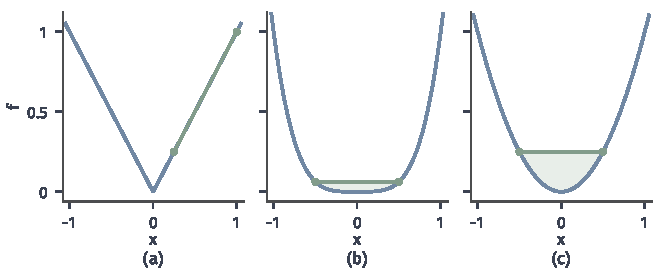
\includegraphics[width=112mm]{figures/05-optimization/01-linear-programming/matplotlib/opt-convexity-gap/figure.pdf}
  \caption{三种弯曲程度下的弦间隔，绿色线段是弦，浅绿区域是间隔。(a)$\lvert x\rvert$在同侧取端点时弦贴着图像，凸但不严格凸。(b)$x^4$严格凸，端点$\pm0.5$的中点处间隔只有$0.0625$。(c)$x^2$是$2$强凸的，同样端点的中点处间隔为$0.25$。}
  \label{fig:opt-convexity-gap}
\end{BookInlineFigure}

\paragraph{目标差控制到解的距离}
强凸性最直接的用途，是把目标值的误差换成位置的误差。

\begin{theorem}[强凸目标的二次增长]
\label{thm:opt-quadratic-growth}
设$\bm{C}$为凸集，$f$在$\bm{C}$上$\mu$强凸，且最优解$\bm{x}^\star$存在。则最优解唯一，并且对所有$\bm{x}\in\bm{C}$，
\begin{equation}
 f(\bm{x})-f^\star\geq\frac{\mu}{2}\lVert\bm{x}-\bm{x}^\star\rVert_2^2.
 \label{eq:opt-quadratic-growth}
\end{equation}
\end{theorem}

\begin{proof}
对$t\in(0,1)$，点$\bm{x}^\star+t(\bm{x}-\bm{x}^\star)$在$\bm{C}$中，目标值不低于$f^\star$。在式~\eqref{eq:opt-strong-convexity}中取$\bm{u}=\bm{x}$，$\bm{v}=\bm{x}^\star$，$\theta=t$，得到
\[
 f^\star\leq tf(\bm{x})+(1-t)f^\star-\frac{\mu}{2}t(1-t)\lVert\bm{x}-\bm{x}^\star\rVert_2^2.
\]

移项后除以$t>0$，得到
\[
 f(\bm{x})-f^\star\geq\frac{\mu}{2}(1-t)\lVert\bm{x}-\bm{x}^\star\rVert_2^2.
\]
令$t\downarrow0$即得式~\eqref{eq:opt-quadratic-growth}。若$\bm{x}$也是最优解，左端为零，迫使$\bm{x}=\bm{x}^\star$。
\end{proof}

证明只用到可行集凸、目标强凸和最优解存在，没有假设解在内部或目标可微。把实例取$\gamma=1$，由式~\eqref{eq:opt-ridge-solution}，$\bm{x}^\star=(2/3,2/3)$，$\mu=1$。取$\bm{x}=\bm{x}^\star+(1,-1)$，两个分量之和不变，所以拟合项不变，目标差全部来自正则项：
\[
 f(\bm{x})-f^\star=\frac12\bigl(\lVert\bm{x}\rVert_2^2-\lVert\bm{x}^\star\rVert_2^2\bigr)=\frac12\cdot2=1.
\]
距离的平方是$2$，式~\eqref{eq:opt-quadratic-growth}的右端也是$1$，在这里取等号，因为位移恰好沿最小特征值的方向。

可行集必须是凸的。$x^2$在$\mathbb{R}$上$2$强凸，但在$C=\{x:\lvert x\rvert\geq1\}$上有两个最小点$\pm1$，两点的目标差为$0$，距离却是$2$。证明中从$\bm{x}^\star$走向$\bm{x}$的线段离开了可行集，那一步就失效了。

表~\ref{tab:opt-convexity-ladder}汇总本节的三级要求及各自多给出的结论。

\begin{BookInlineTable}
  \centering
  \begin{tabular}{@{}lll@{}}
    \toprule
    目标（可行集凸） & 弦下方的间隔 & 结论\\
    \midrule
    凸 & 不小于$0$ & 局部最优即全局最优，解集凸\\
    严格凸 & 大于$0$ & 解至多一个\\
    $\mu$强凸 & 不小于二次量 & 解若存在则唯一，目标差控制距离\\
    \bottomrule
  \end{tabular}
  \caption{沿线段比较的三级要求。每一级都比上一级强，存在性仍需另外保证。}
  \label{tab:opt-convexity-ladder}
\end{BookInlineTable}

\section{最优解的判别}
\label{sec:opt-optimality}

前面的条件都是整体性的：可行集是否紧、目标是否凸。实际计算时，我们手里只有一个候选点，以及它附近的函数值和导数。接下来要弄清：只看这一点的导数信息，能断定什么？不能断定什么？主线讨论无约束的光滑目标，或者可行集内部的点；最后说明受约束时情况怎样改变。

全卷用$\nabla f(\bm{x})$表示梯度，$\nabla^2f(\bm{x})$表示Hessian矩阵。多元函数的梯度、Hessian和Taylor公式，可参考\BookChapterRef{chap:multivariate-differentiation}{卷二第20章“多元函数微分”}。

\paragraph{沿每个方向看}
站在最低点上，朝任何方向迈一小步都不会更低。把这句话变成计算：固定点$\bar{\bm{x}}$和方向$\bm{d}$，只看沿这条直线的一元函数
\[
 \phi(t)=f(\bar{\bm{x}}+t\bm{d}).
\]
链式法则给出它在$t=0$处的导数，即沿$\bm{d}$的\term{方向导数}（directional derivative）：
\begin{equation}
 \phi'(0)=\langle\nabla f(\bar{\bm{x}}),\bm{d}\rangle.
 \label{eq:opt-directional-derivative}
\end{equation}

$\phi'(0)<0$时，沿$\bm{d}$走一小步目标下降，这样的$\bm{d}$称为\term{下降方向}（descent direction）。条件$\langle\nabla f(\bar{\bm{x}}),\bm{d}\rangle<0$说明，只要梯度不为零，下降方向就占据整整半个空间，分界面与梯度垂直，也就是等高线在该点的切线。

用实例~\eqref{eq:opt-ridge-instance}取$\gamma=0.5$算一次。梯度的两个分量是
\[
 \frac{\partial f}{\partial x_1}=x_1+x_2-2+\gamma x_1,\qquad
 \frac{\partial f}{\partial x_2}=x_1+x_2-2+\gamma x_2.
\]
在$\bar{\bm{x}}=(2,0)$处，$\nabla f(\bar{\bm{x}})=(1,0)$。取$\bm{d}=(-1,1)$，由式~\eqref{eq:opt-directional-derivative}，方向导数是$-1$。

直接验证一下。沿这个方向$x_1+x_2$保持为$2$，拟合项为零，于是
\[
 \phi(t)=\frac14\bigl((2-t)^2+t^2\bigr),\qquad\phi'(0)=\frac14\cdot(-4)=-1.
\]
两种算法结果相同。图~\ref{fig:opt-descent-halfplane}中，浅绿半平面是全部下降方向，竖直虚线是等高线在$\bar{\bm{x}}$处的切线。负梯度方向$-\nabla f$是其中的一个，$\bm{d}$是另一个，后者比负梯度更接近指向红色最优解的方向。

\begin{BookInlineFigure}
  \centering
  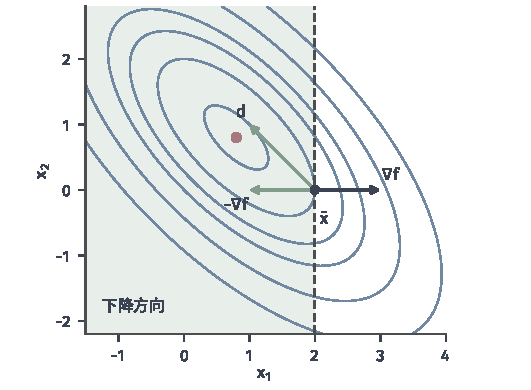
\includegraphics[width=90mm]{figures/05-optimization/01-linear-programming/matplotlib/opt-descent-halfplane/figure.pdf}
  \caption{下降方向构成半平面。蓝线是$f(\bm{x})=\frac12(x_1+x_2-2)^2+\frac14\lVert\bm{x}\rVert_2^2$的等高线，$\bar{\bm{x}}=(2,0)$处的梯度为$(1,0)$。竖直虚线与梯度垂直，浅绿区域的方向都满足$\langle\nabla f(\bar{\bm{x}}),\bm{d}\rangle<0$。绿色箭头是负梯度方向和$\bm{d}=(-1,1)$，红点是最优解$(0.8,0.8)$。}
  \label{fig:opt-descent-halfplane}
\end{BookInlineFigure}

\paragraph{一阶必要条件}
若$\bar{\bm{x}}$是局部最优解，并且各个方向都可以走，就不能有下降方向。半个空间都是下降方向的唯一例外是梯度为零。为了让“各个方向都可以走”成立，下面要求点在可行集内部：称$\bar{\bm{x}}$是$\bm{C}$的\term{内点}（interior point），如果存在$r>0$使$\bm{B}(\bar{\bm{x}},r)\subseteq\bm{C}$。

\begin{theorem}[一阶必要条件]
\label{thm:opt-first-order}
设$\bm{x}^\star$是$\bm{C}$的内点，$f$在$\bm{x}^\star$处可微。若$\bm{x}^\star$是$f$在$\bm{C}$上的局部最优解，则
\begin{equation}
 \nabla f(\bm{x}^\star)=\bm{0}.
 \label{eq:opt-first-order}
\end{equation}
\end{theorem}

\begin{proof}
任取方向$\bm{d}$。$\lvert t\rvert$充分小时，$\bm{x}^\star+t\bm{d}$既在$\bm{C}$内，又在局部最优的邻域内，所以$\phi(t)=f(\bm{x}^\star+t\bm{d})\geq\phi(0)$。

当$t>0$时，$(\phi(t)-\phi(0))/t\geq0$。令$t\downarrow0$，由式~\eqref{eq:opt-directional-derivative}得到
\[
 \langle\nabla f(\bm{x}^\star),\bm{d}\rangle\geq0.
\]
这对任意方向成立。取$\bm{d}=-\nabla f(\bm{x}^\star)$，得到$-\lVert\nabla f(\bm{x}^\star)\rVert_2^2\geq0$，所以梯度为零。
\end{proof}

梯度为零的点称为\term{驻点}（stationary point）。这个条件只是必要的，它在三处不能往下推。第一，驻点不一定是最小点：$x_1^2-x_2^2$在原点有驻点，沿$x_1$轴是最低点，沿$x_2$轴是最高点，这样的驻点称为\term{鞍点}（saddle point）。第二，定理只管内点：例子~\ref{ex:opt-local-global}的全局最优解$x=1.5$在边界上，导数不为零。第三，即使驻点是局部最优，也可能不是全局最优。

下面的二维例子同时展示这几点，后面会反复用到。考虑$\mathbb{R}^2$上的
\begin{equation}
 f(\bm{x})=x_1^3-3x_1+x_2^2.
 \label{eq:opt-cubic}
\end{equation}
令梯度为零：
\[
 \nabla f(\bm{x})=(3x_1^2-3,\ 2x_2)=\bm{0}.
\]
解得两个驻点$(1,0)$和$(-1,0)$。一阶信息到此为止，分不出这两个点的差别。

\paragraph{凸目标的驻点}
凸性能把必要条件变成充分条件。关键在于：凸函数的图像不仅在弦下方，还在每一点切线的上方。切线只用到一个点的函数值和梯度，它若是全局下界，单点信息就能告诉我们远处的目标至少有多大。

\begin{theorem}[一阶支撑不等式]
\label{thm:opt-support}
设$\bm{D}\subseteq\mathbb{R}^n$是开凸集，$f:\bm{D}\to\mathbb{R}$可微。$f$是凸函数，当且仅当对任意$\bm{u},\bm{v}\in\bm{D}$，
\begin{equation}
 f(\bm{v})\geq f(\bm{u})+\langle\nabla f(\bm{u}),\bm{v}-\bm{u}\rangle.
 \label{eq:opt-support}
\end{equation}
\end{theorem}

\begin{proof}
设$f$凸。对$t\in(0,1]$，由式~\eqref{eq:opt-convex-function}，
\[
 f\bigl(\bm{u}+t(\bm{v}-\bm{u})\bigr)\leq(1-t)f(\bm{u})+tf(\bm{v}).
\]
移项并除以$t$，得到
\[
 \frac{f\bigl(\bm{u}+t(\bm{v}-\bm{u})\bigr)-f(\bm{u})}{t}\leq f(\bm{v})-f(\bm{u}).
\]
令$t\downarrow0$，左端趋于方向导数$\langle\nabla f(\bm{u}),\bm{v}-\bm{u}\rangle$，即得式~\eqref{eq:opt-support}。

反过来，设式~\eqref{eq:opt-support}成立。取$\bm{z}=\theta\bm{u}+(1-\theta)\bm{v}$，以$\bm{z}$为切点，分别写出
\[
 f(\bm{u})\geq f(\bm{z})+\langle\nabla f(\bm{z}),\bm{u}-\bm{z}\rangle,\qquad
 f(\bm{v})\geq f(\bm{z})+\langle\nabla f(\bm{z}),\bm{v}-\bm{z}\rangle.
\]
第一式乘$\theta$，第二式乘$1-\theta$，再相加。由$\bm{z}$的定义，
\[
 \theta(\bm{u}-\bm{z})+(1-\theta)(\bm{v}-\bm{z})=\bm{0},
\]
所以内积项抵消，得到式~\eqref{eq:opt-convex-function}。
\end{proof}

图~\ref{fig:opt-support-tangent}对比了两种情形。凸函数的切线（紫色）整条位于图像下方，是全局的下界。非凸函数在$x=0$处的水平切线则位于图像上方的一大段区域，单点信息不能给出下界。

\begin{BookInlineFigure}
  \centering
  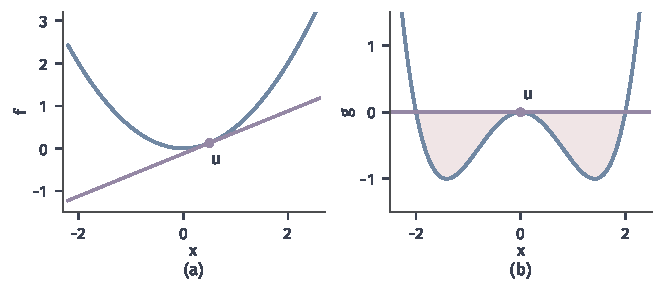
\includegraphics[width=112mm]{figures/05-optimization/01-linear-programming/matplotlib/opt-support-tangent/figure.pdf}
  \caption{切线是否是全局下界。(a)凸函数$f(x)=x^2/2$在$u=1/2$处的紫色切线整条位于图像下方。(b)非凸函数$g(x)=x^4/4-x^2$在$u=0$处的切线是水平线，在$0<\lvert x\rvert<2$时位于图像上方（浅红区域），不是下界。}
  \label{fig:opt-support-tangent}
\end{BookInlineFigure}

把$\nabla f(\bm{x}^\star)=\bm{0}$代入式~\eqref{eq:opt-support}，水平的切平面把最小值钉在切点上。

\begin{theorem}[凸目标驻点的全局最优性]
\label{thm:opt-convex-stationary}
设$\bm{D}$是开凸集，$f:\bm{D}\to\mathbb{R}$凸且可微。则$\bm{x}^\star\in\bm{D}$是$f$在$\bm{D}$上的全局最优解，当且仅当$\nabla f(\bm{x}^\star)=\bm{0}$。
\end{theorem}

\begin{proof}
必要性来自定理~\ref{thm:opt-first-order}，开集中每个点都是内点。充分性：若梯度为零，由式~\eqref{eq:opt-support}，对任意$\bm{v}\in\bm{D}$，
\[
 f(\bm{v})\geq f(\bm{x}^\star)+\langle\bm{0},\bm{v}-\bm{x}^\star\rangle=f(\bm{x}^\star).
\]
\end{proof}

这个结论的价值在于：对凸目标，求解优化问题等价于解方程$\nabla f=\bm{0}$，找到的任何一个解都是全局最优。二次拟合~\eqref{eq:opt-ridge}的梯度是
\begin{equation}
 \nabla f(\bm{x})=\bm{A}^\top(\bm{A}\bm{x}-\bm{b})+\gamma\bm{x},
 \label{eq:opt-ridge-gradient}
\end{equation}
驻点条件就是正规方程
\[
 (\bm{A}^\top\bm{A}+\gamma\bm{I})\bm{x}=\bm{A}^\top\bm{b}.
\]
实例中它化为
\[
 (1+\gamma)x_1+x_2=2,\qquad x_1+(1+\gamma)x_2=2.
\]
两式相减得$\gamma(x_1-x_2)=0$。$\gamma>0$时$x_1=x_2$，解出的正是式~\eqref{eq:opt-ridge-solution}；$\gamma=0$时两式都是$x_1+x_2=2$，解成一条直线。

强凸函数还多一个二次项。设$f$可微且$\mu$强凸。由式~\eqref{eq:opt-strong-equivalent}，$f-\frac{\mu}{2}\lVert\cdot\rVert_2^2$是凸函数，它的梯度是$\nabla f(\bm{x})-\mu\bm{x}$。对它用式~\eqref{eq:opt-support}，其中多出的项可以合并：
\[
 \lVert\bm{v}\rVert_2^2-\lVert\bm{u}\rVert_2^2-2\langle\bm{u},\bm{v}-\bm{u}\rangle=\lVert\bm{v}-\bm{u}\rVert_2^2.
\]
于是得到
\begin{equation}
 f(\bm{v})\geq f(\bm{u})+\langle\nabla f(\bm{u}),\bm{v}-\bm{u}\rangle+\frac{\mu}{2}\lVert\bm{v}-\bm{u}\rVert_2^2.
 \label{eq:opt-strong-support}
\end{equation}

这个不等式顺便补上了强凸目标的存在性。在$\mathbb{R}^n$上取$\bm{u}=\bm{0}$，由柯西不等式，
\[
 f(\bm{v})\geq f(\bm{0})-\lVert\nabla f(\bm{0})\rVert_2\lVert\bm{v}\rVert_2+\frac{\mu}{2}\lVert\bm{v}\rVert_2^2.
\]
右端在$\lVert\bm{v}\rVert_2\to\infty$时趋于$+\infty$，所以$f$强制。可微函数连续，由上一节的结论，最优解存在。再由定理~\ref{thm:opt-quadratic-growth}，最优解唯一。

\paragraph{二阶条件：曲率区分驻点的类型}
一阶条件分不清极小、极大与鞍点，因为驻点处梯度项消失了，函数的变化由下一阶主导。设$f$二阶连续可微，$\nabla f(\bm{x}^\star)=\bm{0}$。由带Lagrange余项的Taylor公式，对小的$\bm{h}$，存在$s\in(0,1)$使
\begin{equation}
 f(\bm{x}^\star+\bm{h})-f(\bm{x}^\star)=\frac12\bm{h}^\top\nabla^2f(\bm{x}^\star+s\bm{h})\bm{h}.
 \label{eq:opt-taylor}
\end{equation}
量$\bm{d}^\top\nabla^2f(\bm{x}^\star)\bm{d}$是函数沿$\bm{d}$方向的曲率：为正时向上弯，为负时向下弯。

\begin{theorem}[二阶条件]
\label{thm:opt-second-order}
设$\bm{x}^\star$是$\bm{C}$的内点，$f$在$\bm{x}^\star$附近二阶连续可微。
\begin{enumerate}
 \item 必要条件：若$\bm{x}^\star$是局部最优解，则$\nabla f(\bm{x}^\star)=\bm{0}$且$\nabla^2f(\bm{x}^\star)$半正定。
 \item 充分条件：若$\nabla f(\bm{x}^\star)=\bm{0}$且$\nabla^2f(\bm{x}^\star)$正定，则$\bm{x}^\star$是严格局部最优解。
\end{enumerate}
\end{theorem}

\begin{proof}
记$\bm{H}=\nabla^2f(\bm{x}^\star)$。先证必要条件，一阶部分即定理~\ref{thm:opt-first-order}。假设某个$\bm{d}$使$\bm{d}^\top\bm{H}\bm{d}<0$。由Hessian的连续性，$\lvert t\rvert$充分小时，对所有$s\in(0,1)$都有
\[
 \bm{d}^\top\nabla^2f(\bm{x}^\star+st\bm{d})\bm{d}<0.
\]
在式~\eqref{eq:opt-taylor}中取$\bm{h}=t\bm{d}$，就得到$f(\bm{x}^\star+t\bm{d})<f(\bm{x}^\star)$，与局部最优矛盾。

再证充分条件。记$\lambda_{\min}>0$为$\bm{H}$的最小特征值，于是
\[
 \bm{h}^\top\bm{H}\bm{h}\geq\lambda_{\min}\lVert\bm{h}\rVert_2^2.
\]
由Hessian的连续性，取足够小的$r>0$，使$\bm{B}(\bm{x}^\star,r)\subseteq\bm{C}$，并且$\lVert\bm{h}\rVert_2<r$时
\[
 \bigl\lVert\nabla^2f(\bm{x}^\star+\bm{h})-\bm{H}\bigr\rVert_2\leq\frac{\lambda_{\min}}{2}.
\]

这样对$\lVert\bm{h}\rVert_2<r$和任意$s\in(0,1)$，二次型至多比$\bm{h}^\top\bm{H}\bm{h}$小$\frac{\lambda_{\min}}{2}\lVert\bm{h}\rVert_2^2$。代入式~\eqref{eq:opt-taylor}，对$\bm{h}\neq\bm{0}$，
\[
 f(\bm{x}^\star+\bm{h})-f(\bm{x}^\star)\geq\frac12\Bigl(\lambda_{\min}-\frac{\lambda_{\min}}{2}\Bigr)\lVert\bm{h}\rVert_2^2=\frac{\lambda_{\min}}{4}\lVert\bm{h}\rVert_2^2>0.
\]
所以$\bm{x}^\star$是严格局部最优解。
\end{proof}

回到式~\eqref{eq:opt-cubic}。它的Hessian是
\[
 \nabla^2f(\bm{x})=\begin{bmatrix}6x_1&0\\0&2\end{bmatrix}.
\]
在$(1,0)$处是$\operatorname{diag}(6,2)$，正定，所以这是严格局部最优解，函数值为$-2$。在$(-1,0)$处是$\operatorname{diag}(-6,2)$，不定，不是局部最优解，也不是局部极大点，而是鞍点，函数值为$2$。

二阶条件到此仍是局部结论。沿$x_1\to-\infty$，$f\to-\infty$，所以这个问题无下界，局部最优点$(1,0)$远不是全局最优。图~\ref{fig:opt-cubic-stationary}中，穿过鞍点的粗等高线围出一个“盆”，$(1,0)$在盆底，翻过鞍点向左，地面一路下降。

\begin{BookInlineFigure}
  \centering
  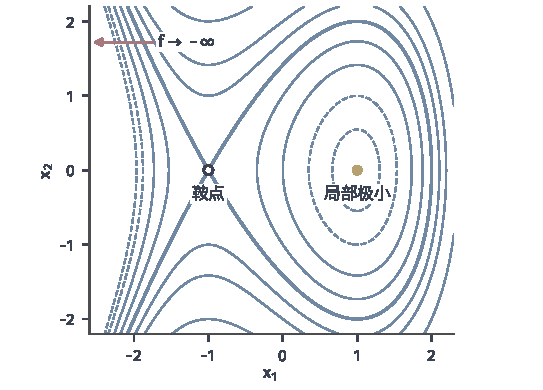
\includegraphics[width=92mm]{figures/05-optimization/01-linear-programming/matplotlib/opt-cubic-stationary/figure.pdf}
  \caption{$f(\bm{x})=x_1^3-3x_1+x_2^2$的等高线，虚线是负值水平。黄点$(1,0)$是严格局部最优解，空心点$(-1,0)$是鞍点，粗线是穿过鞍点的等高线$f=2$。红色箭头所指的左侧目标趋于$-\infty$，所以局部最优解不是全局最优解。}
  \label{fig:opt-cubic-stationary}
\end{BookInlineFigure}

要从局部曲率得到整体结论，就得要求曲率处处非负，这正是凸性的二阶判据。

\begin{theorem}[凸性的二阶判据]
\label{thm:opt-hessian-convex}
设$\bm{D}\subseteq\mathbb{R}^n$是开凸集，$f:\bm{D}\to\mathbb{R}$二阶连续可微。则$f$凸当且仅当$\nabla^2f(\bm{x})$在$\bm{D}$上处处半正定；$f$是$\mu$强凸的当且仅当$\nabla^2f(\bm{x})-\mu\bm{I}$在$\bm{D}$上处处半正定。
\end{theorem}

\begin{proof}
设$f$凸，取$\bm{x}\in\bm{D}$和方向$\bm{h}$。$t$充分小时，由式~\eqref{eq:opt-support}和带Lagrange余项的Taylor公式，存在$s\in(0,1)$使
\[
 0\leq f(\bm{x}+t\bm{h})-f(\bm{x})-t\langle\nabla f(\bm{x}),\bm{h}\rangle=\frac{t^2}{2}\bm{h}^\top\nabla^2f(\bm{x}+st\bm{h})\bm{h}.
\]
除以$t^2/2$，令$t\to0$，由Hessian的连续性得到$\bm{h}^\top\nabla^2f(\bm{x})\bm{h}\geq0$。

反过来，设Hessian处处半正定。对$\bm{u},\bm{v}\in\bm{D}$，令$\psi(t)=f(\bm{u}+t(\bm{v}-\bm{u}))$，则$\psi''\geq0$。由带Lagrange余项的Taylor公式，
\[
 \psi(1)=\psi(0)+\psi'(0)+\frac12\psi''(\xi)\geq\psi(0)+\psi'(0),
\]
这正是式~\eqref{eq:opt-support}，由定理~\ref{thm:opt-support}，$f$凸。

强凸的情形，把上述结论用于$f-\frac{\mu}{2}\lVert\cdot\rVert_2^2$，它的Hessian是$\nabla^2f-\mu\bm{I}$，再用式~\eqref{eq:opt-strong-equivalent}。
\end{proof}

判据要求在整个开凸集上成立，只在单个点检查不能证明函数凸。式~\eqref{eq:opt-cubic}在$(1,0)$处Hessian正定，但在$x_1<0$处有负特征值，所以它不是凸函数，局部最优也就不必是全局最优。二次拟合的Hessian处处等于$\bm{A}^\top\bm{A}+\gamma\bm{I}$，半正定，这与前面用弦算出的结论一致。

\paragraph{退化驻点：二阶也判不了}
定理~\ref{thm:opt-second-order}的两个条件之间留有缺口：Hessian半正定但奇异时，必要条件满足，充分条件不满足，二阶信息不足以判断。这样的驻点称为\term{退化驻点}（degenerate stationary point）。

函数$x_1^2+x_2^4$和$x_1^2+x_2^3$在原点的梯度都为零，Hessian都是$\operatorname{diag}(2,0)$，二阶信息完全相同。前者对$\bm{x}\neq\bm{0}$恒为正，原点是严格最小点，说明正定不是必要的。后者沿$(0,-t)$取值$-t^3<0$，原点不是局部最优解，说明半正定不是充分的。

决定结果的是$x_2$方向的高阶项，这正是Hessian在零特征方向上看不到的信息。图~\ref{fig:opt-stationary-types}中，请注意红色区域是否碰到原点：碰到就说明任意小的邻域里都有更低的点。(c)与(d)的二阶信息相同，红色区域却一有一无。

\begin{BookInlineFigure}
  \centering
  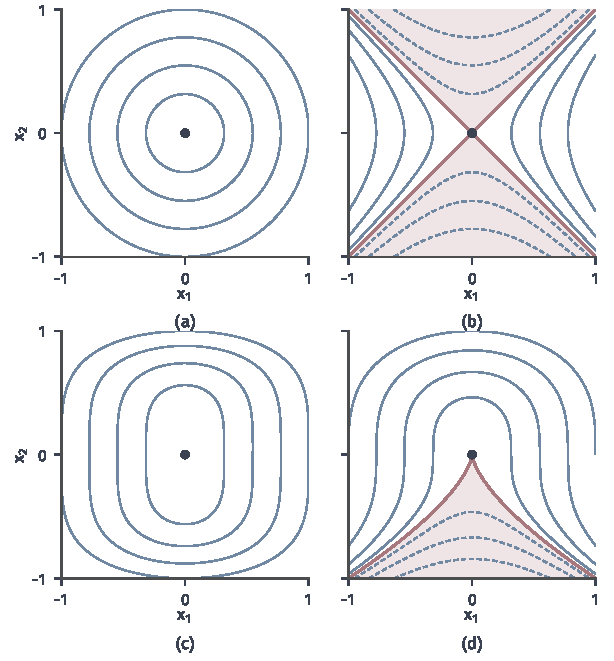
\includegraphics[width=104mm]{figures/05-optimization/01-linear-programming/matplotlib/opt-stationary-types/figure.pdf}
  \caption{原点处四种驻点的等高线，浅红区域是函数值低于$f(\bm{0})=0$的点，虚线是负值水平，红线是零等高线。(a)$x_1^2+x_2^2$，Hessian正定，严格最小点。(b)$x_1^2-x_2^2$，Hessian不定，鞍点。(c)$x_1^2+x_2^4$，Hessian为$\operatorname{diag}(2,0)$，仍是严格最小点。(d)$x_1^2+x_2^3$，Hessian同为$\operatorname{diag}(2,0)$，但原点下方有更低的点，不是局部最优解。}
  \label{fig:opt-stationary-types}
\end{BookInlineFigure}

\paragraph{负曲率方向}
定理~\ref{thm:opt-second-order}必要性的证明还包含一条可以操作的信息。若驻点处存在方向$\bm{d}$使$\bm{d}^\top\nabla^2f(\bm{x}^\star)\bm{d}<0$，就称$\bm{d}$为\term{负曲率方向}（negative curvature direction）。沿它走，一阶变化为零，目标却以二次速度下降。

对$f(\bm{x})=x_1^2-x_2^2$，Hessian是$\operatorname{diag}(2,-2)$。沿单位方向$\bm{d}$，
\[
 f(t\bm{d})=\frac{t^2}{2}\bm{d}^\top\operatorname{diag}(2,-2)\bm{d}=t^2(d_1^2-d_2^2).
\]
图~\ref{fig:opt-saddle-curvature}取三个方向：$\bm{d}_1=(1,0)$曲率为$2$，向上弯；$\bm{d}_2=(1,1)/\sqrt2$曲率为$0$，二阶项恰好消失；$\bm{d}_3=(0,1)$曲率为$-2$，向下弯。站在鞍点上，梯度指不出任何下降方向，Hessian的负特征向量却指出了一条。怎样利用这一点离开鞍点，由第~\ref{chap:saddle-points}章讨论。

\begin{BookInlineFigure}
  \centering
  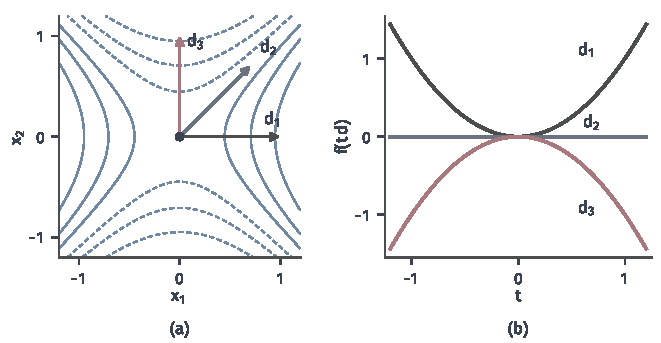
\includegraphics[width=112mm]{figures/05-optimization/01-linear-programming/matplotlib/opt-saddle-curvature/figure.pdf}
  \caption{鞍点处不同方向的曲率。(a)$f(\bm{x})=x_1^2-x_2^2$的等高线（虚线为负值）与三个单位方向。(b)沿这三个方向的一元限制$f(t\bm{d})$：$\bm{d}_1$向上弯，$\bm{d}_2$保持为零，红色的$\bm{d}_3$向下弯，是负曲率方向。}
  \label{fig:opt-saddle-curvature}
\end{BookInlineFigure}

表~\ref{tab:opt-tests}整理到目前为止的判别依据。阅读时要注意“必要”与“充分”的方向，以及结论是局部的还是全局的。

\begin{BookInlineTable}
  \centering
  \begin{tabular}{@{}lll@{}}
    \toprule
    依据 & 性质 & 能得到的结论\\
    \midrule
    $\nabla f=\bm{0}$ & 内点局部最优的必要条件 & 排除非驻点\\
    $\nabla f=\bm{0}$，$\nabla^2f\succeq\bm{0}$ & 局部最优的必要条件 & 进一步排除负曲率点\\
    $\nabla f=\bm{0}$，$\nabla^2f\succ\bm{0}$ & 充分条件，非必要 & 严格局部最优\\
    $\nabla f=\bm{0}$，目标凸 & 充要条件 & 全局最优\\
    \bottomrule
  \end{tabular}
  \caption{无约束光滑目标的判别依据。前三行只看一个点，第四行需要目标的整体性质。}
  \label{tab:opt-tests}
\end{BookInlineTable}

\paragraph{受约束时允许的方向变了}
一阶条件的证明要求$\bm{d}$和$-\bm{d}$都能走。在边界上这个前提不成立，能走的方向变少，要求也相应放宽。称$\bm{d}$是$\bar{\bm{x}}\in\bm{C}$处的\term{可行方向}（feasible direction），如果$t>0$充分小时$\bar{\bm{x}}+t\bm{d}\in\bm{C}$。重复定理~\ref{thm:opt-first-order}证明的前半段，只用$t>0$，就得到：若$\bm{x}^\star$是局部最优解，$f$在该点可微，则对每个可行方向$\bm{d}$，
\begin{equation}
 \langle\nabla f(\bm{x}^\star),\bm{d}\rangle\geq0.
 \label{eq:opt-feasible-direction}
\end{equation}

用资源分配验证。在$\bm{x}^\star=(2,2)$处，两条资源约束取等号，$\bm{d}$可行当且仅当它不增加这两个约束，即
\[
 d_1+d_2\leq0,\qquad 2d_1+d_2\leq0.
\]
目标的梯度是$(-3,-2)$，不等于零。方向导数却可以拆开：
\[
 \langle\nabla f(\bm{x}^\star),\bm{d}\rangle=-3d_1-2d_2=-(d_1+d_2)-(2d_1+d_2)\geq0.
\]

这里的拆分仍然是第~\ref{sec:opt-formulation}节那个“两条约束相加”。图~\ref{fig:opt-boundary-directions}显示了几何含义：$-\nabla f$指向利润增大的方向，它伸出了可行集，而所有绿色的可行方向都和它成钝角或直角。所以$(2,2)$处梯度不为零，却没有“既可行又下降”的方向。

\begin{BookInlineFigure}
  \centering
  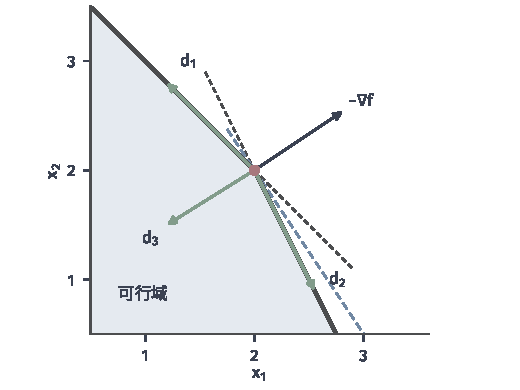
\includegraphics[width=88mm]{figures/05-optimization/01-linear-programming/matplotlib/opt-boundary-directions/figure.pdf}
  \caption{边界上的最优点梯度不必为零。红点是资源分配的最优解$(2,2)$，深灰粗线是两条取等号的约束，蓝色虚线是过该点的等目标线。绿色箭头是可行方向，全部可行方向都夹在$\bm{d}_1=(-1,1)$与$\bm{d}_2=(1,-2)$之间。$-\nabla f=(3,2)$伸出可行集，与每个可行方向的内积都不为正。}
  \label{fig:opt-boundary-directions}
\end{BookInlineFigure}

若$\bm{C}$凸、$f$在包含$\bm{C}$的开凸集上凸且可微，式~\eqref{eq:opt-feasible-direction}对每个$\bm{d}=\bm{y}-\bm{x}^\star$（$\bm{y}\in\bm{C}$）成立时，代入式~\eqref{eq:opt-support}就得到$f(\bm{y})\geq f(\bm{x}^\star)$，所以它也是充分的。

式~\eqref{eq:opt-feasible-direction}还不是一个能直接检验的判据。可行方向可能有无穷多个，曲线边界上甚至可能一个非零的都没有：单位圆周上，沿任何直线都会立刻离开圆周。把它写成关于约束函数的代数条件需要新工具，第~\ref{chap:constrained-optimality}章在明确约束之后建立这些判别。

\section{近似解的评价}
\label{sec:opt-approximate}

前四节讨论的是精确的解。实际计算几乎从不交出精确解：迭代在有限步后停止，浮点运算带来舍入。这就需要回答：拿到一个近似解，怎样说清它好到什么程度？我们会看到，“好”有几种不同的含义，它们回答不同的问题，只在一定条件下可以换算。

\paragraph{算法交出什么}
后面各章的方法都产生一列点。全卷用带括号的上标表示迭代步：$\bm{x}^{(t)}$是第$t$步的点，$t=0,1,\ldots,T$，$T$是总步数。括号把迭代编号与幂区分开，元素下标仍写在下面，如$x_i^{(t)}$。多数方法每一步沿某个方向走一段：
\begin{equation}
 \bm{x}^{(t+1)}=\bm{x}^{(t)}+\alpha^{(t)}\bm{d}^{(t)},
 \label{eq:opt-iteration}
\end{equation}
其中$\bm{d}^{(t)}$是方向，$\alpha^{(t)}>0$是步长。当前点的梯度和Hessian简记为$\bm{g}^{(t)}=\nabla f(\bm{x}^{(t)})$与$\bm{H}^{(t)}=\nabla^2f(\bm{x}^{(t)})$。

算法最后报告的点记为$\hat{\bm{x}}$。本节不关心它怎样得到，只关心怎样评价。要注意$\hat{\bm{x}}$与$\bm{x}^\star$的区别：前者是算法的输出，手里实实在在有；后者是问题的解，我们通常不知道。

\paragraph{目标差}
最直接的指标是目标差
\begin{equation}
 e_f(\hat{\bm{x}})=f(\hat{\bm{x}})-f^\star.
 \label{eq:opt-objective-gap}
\end{equation}
它回答“这个结果比最好的结果差多少”。可行点的目标差非负；若$\hat{\bm{x}}$可行且$e_f(\hat{\bm{x}})\leq\varepsilon$，就称它为$\varepsilon$最优解（$\varepsilon$-optimal solution）。

目标差的麻烦在于$f^\star$通常未知。但只要有一个下界$\ell\leq f^\star$，就有可以计算的上界$e_f(\hat{\bm{x}})\leq f(\hat{\bm{x}})-\ell$。资源分配中，“两条约束相加”给出了下界$\ell=-10$，它不依赖于解出$(2,2)$。对可行点$\hat{\bm{x}}=(1.5,2)$，利润是$8.5$，因此
\[
 f(\hat{\bm{x}})-\ell=-8.5-(-10)=1.5.
\]
这正是上下界夹逼的用处：不知道解在哪里，也能确认当前结果至多差$1.5$。这样的下界怎样系统地构造，是第~\ref{chap:duality}章的主题。

\paragraph{解距离}
第二个指标问位置差多远。设最优解集合$\bm{S}$非空，定义到解集的距离
\begin{equation}
 e_d(\hat{\bm{x}})=\operatorname{dist}(\hat{\bm{x}},\bm{S})=\inf_{\bm{x}\in\bm{S}}\lVert\hat{\bm{x}}-\bm{x}\rVert_2.
 \label{eq:opt-solution-distance}
\end{equation}
解唯一时，它就是$\lVert\hat{\bm{x}}-\bm{x}^\star\rVert_2$。

解不唯一时要注意参照对象。实例~\eqref{eq:opt-ridge-instance}取$\gamma=0$，点$(11,-9)$在直线$x_1+x_2=2$上，它本身就是最优解，到解集的距离为$0$。若心里的“正确系数”是$(1,1)$，两者却相距$\lVert(10,-10)\rVert_2\approx14.1$。把解距离写成到某一个解的距离，就在问题没有提供信息的地方提了要求。

\paragraph{梯度大小}
前两个指标都含有未知量，第三个可以直接算：
\begin{equation}
 e_g(\hat{\bm{x}})=\lVert\nabla f(\hat{\bm{x}})\rVert_2.
 \label{eq:opt-gradient-size}
\end{equation}
由第~\ref{sec:opt-optimality}节，无约束时局部最优解的梯度为零，所以梯度大小可以作为一种缺口的度量。满足$e_g(\hat{\bm{x}})\leq\varepsilon$的点称为$\varepsilon$驻点（$\varepsilon$-stationary point）。

梯度小却不等于接近解。图~\ref{fig:opt-flat-gradient}(a)比较$f_1(x)=0.005x^2$与$f_2(x)=0.5x^2$，两者的最小点都是$0$。在$x=10$处$f_1'=0.1$，在$x=0.1$处$f_2'=0.1$，梯度一样大。前者的目标差是$0.5$，距离是$10$；后者分别是$0.005$和$0.1$。原因在曲率：$f_1$的二阶导数只有$0.01$，地形太平，坡度很小时离谷底仍然很远。

\begin{BookInlineFigure}
  \centering
  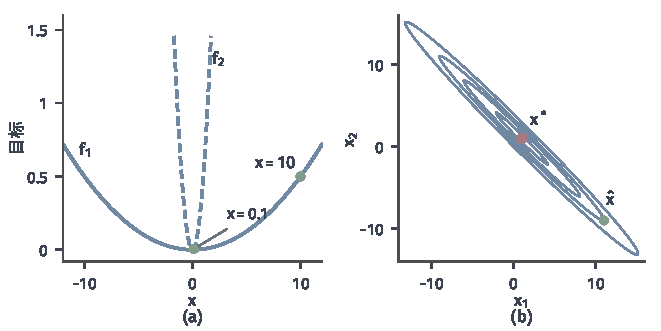
\includegraphics[width=112mm]{figures/05-optimization/01-linear-programming/matplotlib/opt-flat-gradient/figure.pdf}
  \caption{小梯度与小误差。(a)平坦的$f_1(x)=0.005x^2$（实线）在$x=10$处与陡峭的$f_2(x)=0.5x^2$（虚线）在$x=0.1$处导数都是$0.1$，目标差和距离却相差约两个量级。(b)拟合实例取$\gamma=0.01$，蓝线是目标差等于$0.1,0.5,1,2$的等高线，沿$(1,-1)$方向被拉得极长。绿点$\hat{\bm{x}}=(11,-9)$的梯度大小约为$0.142$，到红点$\bm{x}^\star$的距离约为$14.1$。}
  \label{fig:opt-flat-gradient}
\end{BookInlineFigure}

二维的情形更说明问题。实例~\eqref{eq:opt-ridge-instance}取$\gamma=0.01$，由式~\eqref{eq:opt-ridge-solution}，解和最优值是
\[
 \bm{x}^\star\approx(0.995,0.995),\qquad f^\star\approx0.00995.
\]
取$\hat{\bm{x}}=(11,-9)$。两分量之和为$2$，拟合项为零，于是目标值和梯度分别是
\[
 f(\hat{\bm{x}})=0.005\cdot(121+81)=1.01,\qquad\nabla f(\hat{\bm{x}})=(0.11,-0.09).
\]

三个指标的数值是
\[
 e_f\approx1.000,\qquad e_d\approx14.14,\qquad e_g\approx0.142.
\]
观测已经完美拟合，梯度也不大，点却在长沟里离解很远。图~\ref{fig:opt-flat-gradient}(b)的长沟就是强凸常数$\mu=0.01$很小的样子。

驻点还有另一重不足：非凸目标的驻点可以根本不是局部最优解。式~\eqref{eq:opt-cubic}的鞍点$(-1,0)$梯度为零，$e_g=0$，而这个问题甚至没有下界。所以“算法找到驻点”和“算法找到解”是两个强度不同的结论。

\paragraph{三种指标的容差集合}
把三个指标都限定在同一个$\varepsilon$以内，得到三个不同形状的区域。以二次目标为例，记位移$\bm{w}=\bm{x}-\bm{x}^\star$。由$\nabla f(\bm{x}^\star)=\bm{0}$，三个区域分别是
\[
 \tfrac12\bm{w}^\top\bm{H}\bm{w}\leq\varepsilon,\qquad
 \lVert\bm{w}\rVert_2\leq\varepsilon,\qquad
 \lVert\bm{H}\bm{w}\rVert_2\leq\varepsilon.
\]
图~\ref{fig:opt-tolerance-regions}取实例$\gamma=0.1$，$\varepsilon=0.1$。圆很小；目标差的椭圆沿平坦方向半轴为$\sqrt{2\varepsilon/\gamma}\approx1.41$；梯度的椭圆沿平坦方向半轴为$\varepsilon/\gamma=1$，沿陡峭方向只有$\varepsilon/(2+\gamma)\approx0.048$。

三个区域互不包含，所以“达到精度$\varepsilon$”必须说明用的是哪个指标。沿平坦方向，目标差和梯度都很宽容；沿陡峭方向，梯度最严格。

\begin{BookInlineFigure}
  \centering
  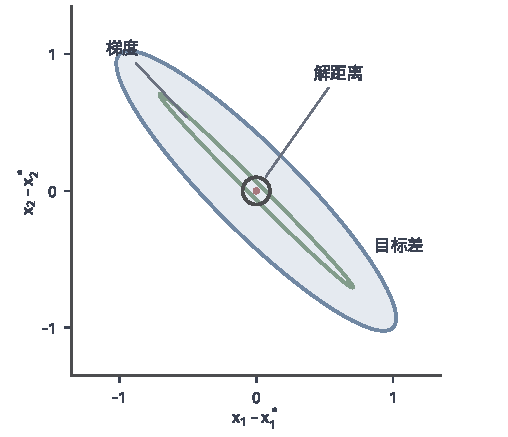
\includegraphics[width=86mm]{figures/05-optimization/01-linear-programming/matplotlib/opt-tolerance-regions/figure.pdf}
  \caption{同一个$\varepsilon=0.1$下三种指标的容差集合，横纵轴是相对于$\bm{x}^\star$的位移，目标取$\gamma=0.1$的拟合实例，$\bm{H}$的特征值为$0.1$和$2.1$。蓝色椭圆内目标差不超过$\varepsilon$，绿色椭圆内梯度大小不超过$\varepsilon$，深灰色小圆内解距离不超过$\varepsilon$。}
  \label{fig:opt-tolerance-regions}
\end{BookInlineFigure}

\paragraph{换算的条件：曲率的上下界}
前面的例子都指向曲率。把它变成定量结论，需要两个常数：曲率的下界$\mu$和上界$L$。全卷用$L$表示光滑常数，用$\kappa=L/\mu$表示条件数。这里先在二阶可微的情形下引入，用$\bm{A}\preceq\bm{B}$表示$\bm{B}-\bm{A}$半正定。第~\ref{chap:smooth-foundations}章将把$L$推广到只要求梯度Lipschitz连续的函数。

\begin{theorem}[三种误差的换算]
\label{thm:opt-error-conversions}
设$f:\mathbb{R}^n\to\mathbb{R}$二阶连续可微，且存在$0<\mu\leq L$，使对所有$\bm{x}$，
\begin{equation}
 \mu\bm{I}\preceq\nabla^2f(\bm{x})\preceq L\bm{I}.
 \label{eq:opt-curvature-bounds}
\end{equation}
则$f$有唯一最优解$\bm{x}^\star$，并且对任意$\bm{x}$，
\begin{equation}
 \begin{gathered}
 \frac{\mu}{2}e_d^2\leq e_f\leq\frac{L}{2}e_d^2,\qquad
 \mu e_d\leq e_g\leq Le_d,\\
 \frac{1}{2L}e_g^2\leq e_f\leq\frac{1}{2\mu}e_g^2.
 \end{gathered}
 \label{eq:opt-error-conversions}
\end{equation}
\end{theorem}

\begin{proof}
由定理~\ref{thm:opt-hessian-convex}，$f$是$\mu$强凸的，由第~\ref{sec:opt-optimality}节的结论，最优解存在且唯一。记$\bm{w}=\bm{x}-\bm{x}^\star$，$e_d=\lVert\bm{w}\rVert_2$。

第一组：由式~\eqref{eq:opt-taylor}，存在$s\in(0,1)$使
\[
 e_f=\frac12\bm{w}^\top\nabla^2f(\bm{x}^\star+s\bm{w})\bm{w}.
\]
再用式~\eqref{eq:opt-curvature-bounds}夹住二次型，即得。

第二组：由$\nabla f(\bm{x}^\star)=\bm{0}$和微积分基本定理，
\[
 \nabla f(\bm{x})=\bm{B}\bm{w},\qquad\bm{B}=\int_0^1\nabla^2f(\bm{x}^\star+s\bm{w})\,\mathrm{d}s.
\]
$\bm{B}$对称，其二次型是被积函数二次型的积分，所以特征值都在$[\mu,L]$内，于是
\[
 \mu\lVert\bm{w}\rVert_2\leq\lVert\bm{B}\bm{w}\rVert_2\leq L\lVert\bm{w}\rVert_2.
\]

第三组的右半：在式~\eqref{eq:opt-strong-support}中取$\bm{u}=\bm{x}$，右端是$\bm{v}$的二次函数，在$\bm{v}=\bm{x}-\nabla f(\bm{x})/\mu$处最小。所以对所有$\bm{v}$，
\[
 f(\bm{v})\geq f(\bm{x})-\frac{1}{2\mu}\lVert\nabla f(\bm{x})\rVert_2^2.
\]
取$\bm{v}=\bm{x}^\star$即得$e_f\leq e_g^2/(2\mu)$。

第三组的左半：由Taylor公式和$\nabla^2f\preceq L\bm{I}$，对任意$\bm{p}$有
\[
 f(\bm{x}+\bm{p})\leq f(\bm{x})+\langle\nabla f(\bm{x}),\bm{p}\rangle+\frac{L}{2}\lVert\bm{p}\rVert_2^2.
\]
取$\bm{p}=-\nabla f(\bm{x})/L$，得到
\[
 f^\star\leq f\Bigl(\bm{x}-\frac{1}{L}\nabla f(\bm{x})\Bigr)\leq f(\bm{x})-\frac{1}{2L}\lVert\nabla f(\bm{x})\rVert_2^2.
\]
移项即得$e_f\geq e_g^2/(2L)$。
\end{proof}

图~\ref{fig:opt-metric-conversions}把式~\eqref{eq:opt-error-conversions}画成一张换算图，每条箭头表示“已知箭尾的量，可以控制箭头的量”。凡用到$\mu$的箭头，都是从目标值或梯度推断位置，需要下弯曲率；用到$L$的箭头，是从位置推断目标值或梯度，需要上弯曲率有限。

\begin{BookInlineFigure}
  \centering
  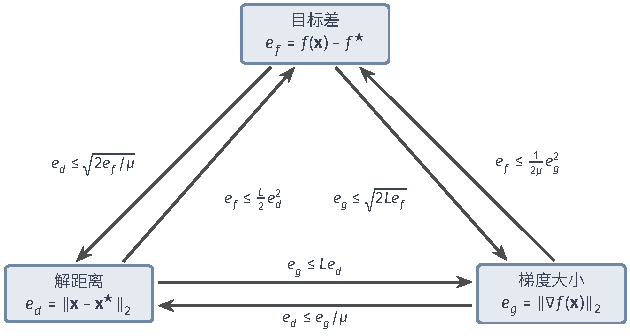
\includegraphics[width=106.74mm]{figures/05-optimization/01-linear-programming/tikz/opt-metric-conversions/figure.pdf}
  \caption{无约束时三种误差的换算，条件是$\mu\bm{I}\preceq\nabla^2f\preceq L\bm{I}$。箭头从已知量指向被控制的量。可计算的只有右下角的梯度大小，它指向其余两个量的两条箭头都依赖$\mu$。}
  \label{fig:opt-metric-conversions}
\end{BookInlineFigure}

用$\gamma=0.01$的实例代入。此时$\mu=0.01$，$L=2.01$，$\kappa=201$。对$\hat{\bm{x}}=(11,-9)$，右半边的两个上界是
\[
 e_f\leq\frac{e_g^2}{2\mu}\approx\frac{0.0202}{0.02}=1.01,\qquad
 e_d\leq\frac{e_g}{\mu}\approx14.2.
\]
实际值是$1.000$和$14.14$，两个界都很贴近，因为$\hat{\bm{x}}-\bm{x}^\star$几乎沿着平坦方向。而梯度约$0.142$这个数看起来很小，放大$1/\mu=100$倍后才是真实的距离。

两个常数不能互相替代，缺了一个，相应的箭头就断了。$\mu$接近零时，梯度几乎不提供关于目标差和距离的信息。$L$不存在时，距离小也不能保证梯度小：$\lvert x\rvert$在任意靠近$0$的点$x\neq0$处，梯度大小都是$1$。$\kappa$大表示两个方向的曲率差得远，同一个$e_d$对应的$e_g$可以相差$\kappa$倍。

\paragraph{有约束时：可行性}
定理~\ref{thm:opt-error-conversions}只针对无约束问题。有约束时，算法的输出可能不满足约束，目标差本身也就失去了意义。用\term{可行性残差}（feasibility residual）度量违反的程度：
\begin{equation}
 r_{\mathrm{feas}}(\hat{\bm{x}})=\max\Bigl\{\max_{i}\,\max\{g_i(\hat{\bm{x}}),0\},\ \max_{j}\,\lvert h_j(\hat{\bm{x}})\rvert\Bigr\}.
 \label{eq:opt-feasibility-residual}
\end{equation}
可行点的残差为零，残差大于零的点违反了至少一条约束。

资源分配中取点$\tilde{\bm{x}}=(2.1,2)$，它违反了两条资源约束：
\[
 g_1(\tilde{\bm{x}})=0.1,\qquad g_2(\tilde{\bm{x}})=0.2,\qquad r_{\mathrm{feas}}(\tilde{\bm{x}})=0.2.
\]
它的利润是$10.3$，比最优利润还高，也就是$f(\tilde{\bm{x}})-f^\star=-0.3<0$。多出来的利润并不是好事，它来自多用的资源。把两条约束相加的论证用在这里，利润至多超出$g_1+g_2=0.3$，恰好等于$0.3$。

反过来，可行点$(0,0)$的残差为零，利润却是$0$，目标差为$10$。图~\ref{fig:opt-feasibility-gap}中，绿点可行但利润不足，红叉利润过高但不可行。所以只报告目标值或只报告可行性都不够，两者要一起报告。

\begin{BookInlineFigure}
  \centering
  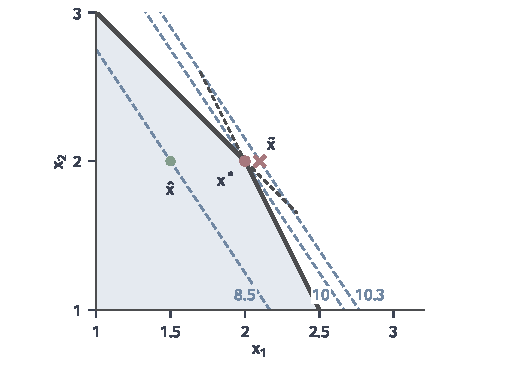
\includegraphics[width=88mm]{figures/05-optimization/01-linear-programming/matplotlib/opt-feasibility-gap/figure.pdf}
  \caption{目标值与可行性要一起看。浅蓝区域是资源分配的部分可行集，蓝色虚线旁的数字是利润。绿点$\hat{\bm{x}}=(1.5,2)$可行，利润$8.5$；红点$\bm{x}^\star=(2,2)$是最优解，利润$10$；红叉$\tilde{\bm{x}}=(2.1,2)$利润$10.3$，高于最优值，但违反了两条资源约束。}
  \label{fig:opt-feasibility-gap}
\end{BookInlineFigure}

约束的数值量纲也影响残差。把“工时”的单位换成分钟，同一条约束乘以$60$，残差也放大$60$倍，可行集却没有变。比较之前要先把约束的尺度说清楚。

\paragraph{有约束时：最优性残差}
第~\ref{sec:opt-optimality}节的图~\ref{fig:opt-boundary-directions}说明，有约束时梯度大小不再是合适的度量：最优解处的梯度不必为零。\term{最优性残差}（optimality residual）指这样一类量：在当前点可以计算，并且恰好在一阶条件成立时为零。无约束时它就是梯度大小。

一个能手算的情形是盒约束$\bm{C}=\{\bm{x}:l_i\leq x_i\leq u_i\}$，上下界允许取无穷。记$\Pi_{\bm{C}}$为逐坐标截断到$[l_i,u_i]$的投影，定义
\begin{equation}
 \bm{r}(\bm{x})=\bm{x}-\Pi_{\bm{C}}\bigl(\bm{x}-\nabla f(\bm{x})\bigr).
 \label{eq:opt-projected-residual}
\end{equation}
逐坐标看，记$g_i$为此处的第$i$个偏导数：$x_i$严格在区间内部时，$r_i=0$要求$g_i=0$；$x_i=l_i$时，$r_i=0$只要求$g_i\geq0$；$x_i=u_i$时，只要求$g_i\leq0$。这正是可行方向条件~\eqref{eq:opt-feasible-direction}逐坐标的写法。

取实例$\gamma=0.5$，加约束$x_1\geq1.2$。解在边界上：固定$x_1=1.2$，对$x_2$最小化得$x_2=8/15$，点$\bm{x}^\star=(1.2,8/15)$。此处的梯度由式~\eqref{eq:opt-ridge-gradient}算得
\[
 \nabla f(\bm{x}^\star)=\Bigl(\frac13,\ 0\Bigr).
\]
梯度不为零，但第一个坐标在下界上，偏导数非负，$\bm{r}(\bm{x}^\star)=\bm{0}$。这个问题是凸的，由上一节的充分性，$\bm{x}^\star$确实是最优解。

再看一个不是解的可行点$\hat{\bm{x}}=(1.5,0.5)$。此处$\nabla f(\hat{\bm{x}})=(0.75,0.25)$，先走一步再截断：
\[
 \hat{\bm{x}}-\nabla f(\hat{\bm{x}})=(0.75,0.25),\qquad
 \Pi_{\bm{C}}(0.75,0.25)=(1.2,0.25).
\]
所以$\bm{r}(\hat{\bm{x}})=(0.3,0.25)$，范数约为$0.39$。这个残差告诉我们，点还没有满足一阶条件。

一般约束的最优性残差要用到约束梯度的组合，由第~\ref{chap:constrained-optimality}章建立；非光滑目标没有梯度，相应的量由第~\ref{chap:nonsmooth-composite-optimization}章定义。这里只需记住它的职责：在不知道解的情况下，度量当前点离一阶条件还差多少。

\paragraph{精度标准}
表~\ref{tab:opt-metrics}汇总这些指标。后续各章陈述结果时，都要说清用的是哪一个。

\begin{table*}[!htbp]
  \centering
  \begin{tabular}{@{}llll@{}}
    \toprule
    指标 & 回答的问题 & 能否直接计算 & 换算所需条件\\
    \midrule
    目标差$e_f$ & 结果比最好差多少 & 需要$f^\star$或其下界 & 可行点；$\mu$可换成距离，$L$可换成梯度\\
    解距离$e_d$ & 位置差多远 & 需要解集 & 解不唯一时参照解集；$L$可换成目标差和梯度\\
    梯度大小$e_g$ & 局部还有多少下降余地 & 能 & 无约束；$\mu$才能换成目标差和距离\\
    可行性残差$r_{\mathrm{feas}}$ & 违反约束多少 & 能 & 依赖约束的尺度\\
    最优性残差 & 离一阶条件还差多少 & 能 & 凸问题中才对应全局最优\\
    \bottomrule
  \end{tabular}
  \caption{近似解的评价指标。前三项针对无约束或已知可行的点，后两项用于约束问题；换算条件的含义见定理~\ref{thm:opt-error-conversions}。}
  \label{tab:opt-metrics}
\end{table*}

阈值的取法也要交代。绝对标准$e_g\leq\varepsilon$依赖目标的尺度：把$f$整体乘以$100$，解不变，梯度却放大$100$倍，同一个$\varepsilon$的严格程度就变了。所以实践中常用相对标准，例如
\begin{equation}
 \lVert\bm{g}^{(t)}\rVert_2\leq\varepsilon\,\max\bigl\{1,\lVert\bm{g}^{(0)}\rVert_2\bigr\}.
 \label{eq:opt-relative-stopping}
\end{equation}

评价方法与决定停止是两种场合。比较方法时，常对同一问题先用高精度方法算出参照值$f^\star$，再看目标差随计算量的变化；参照值本身也有误差，应当说明怎样得到。实际求解时$f^\star$未知，只能依据可计算的残差决定何时停止，而残差小对目标差意味着什么，取决于$\mu$这样的条件。

最后要区分算法的结论。说“迭代收敛到驻点”“输出满足$e_g\leq\varepsilon$”“输出是$\varepsilon$最优解”，是三个强度依次上升的陈述，中间隔着凸性或曲率下界这样的条件。迭代次数与每步代价怎样计入比较，由第~\ref{chap:smooth-foundations}章规定。

\section{本章小结}
\label{sec:opt-summary}

本章把“在允许的选择里找最好的”拆成了几个分别回答的问题。写一个优化问题要同时给出决策变量、目标函数和可行集。最优值是下确界，最优解是取得它的可行点，两者可以分离：问题可能不可行、无下界，或最优值有限却未被达到。局部最优只和附近的可行点比较，全局最优和所有可行点比较。约束指标函数把约束并入目标而不改变问题，普通指示函数和有限惩罚则不能这样用。

存在性靠最小化序列的三关：留得住、极限合法、比较传得到。紧性通过前两关，下半连续通过第三关，无界可行集用紧下水平集或强制性处理。解的性质靠线段比较：凸性使局部最优成为全局最优，严格凸使解至多一个，强凸使目标差控制到解的距离。

判别依赖一个点的导数信息。一阶和二阶条件在内点上区分驻点、局部最优和鞍点，它们本身是局部的；只有目标凸时，驻点才是全局最优。边界上的最优点梯度可以不为零，因为允许的方向变少了。

两个贯穿的例子展示了这些问题怎样得到回答。资源分配的可行集是有界多面体，解存在；把两条资源约束相加，同时得到下界和达到它的点$(2,2)$。二次拟合的$\gamma>0$让目标强制，又让Hessian正定，解存在且唯一，目标差可以换成距离；$\gamma=0$且$\bm{A}$秩亏时，目标不再强制，解仍存在，却成了一条直线。

表~\ref{tab:opt-summary}汇总各结论所需的条件，表中均为充分条件，反例列说明去掉条件或反向推断时的后果。

\begin{table*}[!htbp]
\centering
\small
\begin{tabularx}{\linewidth}{@{}>{\RaggedRight\arraybackslash}p{24mm}>{\RaggedRight\arraybackslash}X>{\RaggedRight\arraybackslash}X>{\RaggedRight\arraybackslash}X@{}}
\toprule
问题 & 充分条件 & 结论 & 反例或边界 \\
\midrule
最优解是否存在 & 可行集非空紧，目标下半连续且有有限值；或某个下水平集非空紧 & 最优值有限且被达到 & $(0,1]$上的$x$；$[1,\infty)$上的$1/x$；在$0$处跳高的函数 \\
局部是否即全局 & 可行集凸，目标凸 & 局部最优解都是全局最优解，解集凸 & 例子中的四次函数；$[-3,-1]\cup[1,3]$上的$(x-2)^2$ \\
解是否唯一 & 可行集凸，目标严格凸，解存在 & 解唯一 & $e^x$严格凸而无最小点；$\lvert x\rvert$与资源分配有唯一解而不严格凸 \\
目标差能否换成距离 & 可行集凸，目标$\mu$强凸，解存在 & $f(\bm{x})-f^\star\geq\frac{\mu}{2}\lVert\bm{x}-\bm{x}^\star\rVert_2^2$ & 非凸可行集$\{\lvert x\rvert\geq1\}$上的$x^2$ \\
内点能否用梯度判别 & 可微；开凸集上目标凸 & 局部最优必有$\nabla f=\bm{0}$；凸时$\nabla f=\bm{0}$即全局最优 & 鞍点；边界最优点的导数可不为零 \\
驻点是否局部最优 & 二阶连续可微，Hessian正定 & 严格局部最优解 & $x_1^2+x_2^4$（正定非必要）；$x_1^2+x_2^3$（半正定不充分）\\
小梯度是否表示小误差 & $\mu\bm{I}\preceq\nabla^2f\preceq L\bm{I}$，无约束 & $e_f\leq e_g^2/(2\mu)$，$e_d\leq e_g/\mu$ & 平坦目标$0.005x^2$；$\gamma=0.01$的拟合实例 \\
\bottomrule
\end{tabularx}
\caption{本章主要问题、充分条件与边界。}
\label{tab:opt-summary}
\end{table*}

算法的输出和问题的解是两回事。输出$\hat{\bm{x}}$由目标差、解距离、梯度大小、可行性残差和最优性残差分别衡量，它们回答不同的问题，只有在曲率上下界这样的条件下才能换算，系数随$1/\mu$放大。

本章没有构造任何算法。从下一章起，线性规划把这些语言用在最具体的模型上：可行集是多面体，解在顶点中寻找，“给约束配权重再相加”发展成可以核对的最优性证书。

